% Options for packages loaded elsewhere
\PassOptionsToPackage{unicode}{hyperref}
\PassOptionsToPackage{hyphens}{url}
\PassOptionsToPackage{dvipsnames,svgnames,x11names}{xcolor}
%
\documentclass[
  a4paper,
]{book}

\usepackage{amsmath,amssymb}
\usepackage{iftex}
\ifPDFTeX
  \usepackage[T1]{fontenc}
  \usepackage[utf8]{inputenc}
  \usepackage{textcomp} % provide euro and other symbols
\else % if luatex or xetex
  \usepackage{unicode-math}
  \defaultfontfeatures{Scale=MatchLowercase}
  \defaultfontfeatures[\rmfamily]{Ligatures=TeX,Scale=1}
\fi
\usepackage{lmodern}
\ifPDFTeX\else  
    % xetex/luatex font selection
\fi
% Use upquote if available, for straight quotes in verbatim environments
\IfFileExists{upquote.sty}{\usepackage{upquote}}{}
\IfFileExists{microtype.sty}{% use microtype if available
  \usepackage[]{microtype}
  \UseMicrotypeSet[protrusion]{basicmath} % disable protrusion for tt fonts
}{}
\makeatletter
\@ifundefined{KOMAClassName}{% if non-KOMA class
  \IfFileExists{parskip.sty}{%
    \usepackage{parskip}
  }{% else
    \setlength{\parindent}{0pt}
    \setlength{\parskip}{6pt plus 2pt minus 1pt}}
}{% if KOMA class
  \KOMAoptions{parskip=half}}
\makeatother
\usepackage{xcolor}
\usepackage[paperwidth=8.27in,paperheight=11.69in,left=1.25in,textwidth=
5.25in,top=1.00in,textheight=8.25in]{geometry}
\setlength{\emergencystretch}{3em} % prevent overfull lines
\setcounter{secnumdepth}{5}
% Make \paragraph and \subparagraph free-standing
\makeatletter
\ifx\paragraph\undefined\else
  \let\oldparagraph\paragraph
  \renewcommand{\paragraph}{
    \@ifstar
      \xxxParagraphStar
      \xxxParagraphNoStar
  }
  \newcommand{\xxxParagraphStar}[1]{\oldparagraph*{#1}\mbox{}}
  \newcommand{\xxxParagraphNoStar}[1]{\oldparagraph{#1}\mbox{}}
\fi
\ifx\subparagraph\undefined\else
  \let\oldsubparagraph\subparagraph
  \renewcommand{\subparagraph}{
    \@ifstar
      \xxxSubParagraphStar
      \xxxSubParagraphNoStar
  }
  \newcommand{\xxxSubParagraphStar}[1]{\oldsubparagraph*{#1}\mbox{}}
  \newcommand{\xxxSubParagraphNoStar}[1]{\oldsubparagraph{#1}\mbox{}}
\fi
\makeatother


\providecommand{\tightlist}{%
  \setlength{\itemsep}{0pt}\setlength{\parskip}{0pt}}\usepackage{longtable,booktabs,array}
\usepackage{calc} % for calculating minipage widths
% Correct order of tables after \paragraph or \subparagraph
\usepackage{etoolbox}
\makeatletter
\patchcmd\longtable{\par}{\if@noskipsec\mbox{}\fi\par}{}{}
\makeatother
% Allow footnotes in longtable head/foot
\IfFileExists{footnotehyper.sty}{\usepackage{footnotehyper}}{\usepackage{footnote}}
\makesavenoteenv{longtable}
\usepackage{graphicx}
\makeatletter
\newsavebox\pandoc@box
\newcommand*\pandocbounded[1]{% scales image to fit in text height/width
  \sbox\pandoc@box{#1}%
  \Gscale@div\@tempa{\textheight}{\dimexpr\ht\pandoc@box+\dp\pandoc@box\relax}%
  \Gscale@div\@tempb{\linewidth}{\wd\pandoc@box}%
  \ifdim\@tempb\p@<\@tempa\p@\let\@tempa\@tempb\fi% select the smaller of both
  \ifdim\@tempa\p@<\p@\scalebox{\@tempa}{\usebox\pandoc@box}%
  \else\usebox{\pandoc@box}%
  \fi%
}
% Set default figure placement to htbp
\def\fps@figure{htbp}
\makeatother
% definitions for citeproc citations
\NewDocumentCommand\citeproctext{}{}
\NewDocumentCommand\citeproc{mm}{%
  \begingroup\def\citeproctext{#2}\cite{#1}\endgroup}
\makeatletter
 % allow citations to break across lines
 \let\@cite@ofmt\@firstofone
 % avoid brackets around text for \cite:
 \def\@biblabel#1{}
 \def\@cite#1#2{{#1\if@tempswa , #2\fi}}
\makeatother
\newlength{\cslhangindent}
\setlength{\cslhangindent}{1.5em}
\newlength{\csllabelwidth}
\setlength{\csllabelwidth}{3em}
\newenvironment{CSLReferences}[2] % #1 hanging-indent, #2 entry-spacing
 {\begin{list}{}{%
  \setlength{\itemindent}{0pt}
  \setlength{\leftmargin}{0pt}
  \setlength{\parsep}{0pt}
  % turn on hanging indent if param 1 is 1
  \ifodd #1
   \setlength{\leftmargin}{\cslhangindent}
   \setlength{\itemindent}{-1\cslhangindent}
  \fi
  % set entry spacing
  \setlength{\itemsep}{#2\baselineskip}}}
 {\end{list}}
\usepackage{calc}
\newcommand{\CSLBlock}[1]{\hfill\break\parbox[t]{\linewidth}{\strut\ignorespaces#1\strut}}
\newcommand{\CSLLeftMargin}[1]{\parbox[t]{\csllabelwidth}{\strut#1\strut}}
\newcommand{\CSLRightInline}[1]{\parbox[t]{\linewidth - \csllabelwidth}{\strut#1\strut}}
\newcommand{\CSLIndent}[1]{\hspace{\cslhangindent}#1}

\makeatletter
\@ifpackageloaded{tcolorbox}{}{\usepackage[skins,breakable]{tcolorbox}}
\@ifpackageloaded{fontawesome5}{}{\usepackage{fontawesome5}}
\definecolor{quarto-callout-color}{HTML}{909090}
\definecolor{quarto-callout-note-color}{HTML}{0758E5}
\definecolor{quarto-callout-important-color}{HTML}{CC1914}
\definecolor{quarto-callout-warning-color}{HTML}{EB9113}
\definecolor{quarto-callout-tip-color}{HTML}{00A047}
\definecolor{quarto-callout-caution-color}{HTML}{FC5300}
\definecolor{quarto-callout-color-frame}{HTML}{acacac}
\definecolor{quarto-callout-note-color-frame}{HTML}{4582ec}
\definecolor{quarto-callout-important-color-frame}{HTML}{d9534f}
\definecolor{quarto-callout-warning-color-frame}{HTML}{f0ad4e}
\definecolor{quarto-callout-tip-color-frame}{HTML}{02b875}
\definecolor{quarto-callout-caution-color-frame}{HTML}{fd7e14}
\makeatother
\makeatletter
\@ifpackageloaded{bookmark}{}{\usepackage{bookmark}}
\makeatother
\makeatletter
\@ifpackageloaded{caption}{}{\usepackage{caption}}
\AtBeginDocument{%
\ifdefined\contentsname
  \renewcommand*\contentsname{Índice}
\else
  \newcommand\contentsname{Índice}
\fi
\ifdefined\listfigurename
  \renewcommand*\listfigurename{Lista de Figuras}
\else
  \newcommand\listfigurename{Lista de Figuras}
\fi
\ifdefined\listtablename
  \renewcommand*\listtablename{Lista de Tabelas}
\else
  \newcommand\listtablename{Lista de Tabelas}
\fi
\ifdefined\figurename
  \renewcommand*\figurename{Figura}
\else
  \newcommand\figurename{Figura}
\fi
\ifdefined\tablename
  \renewcommand*\tablename{Tabela}
\else
  \newcommand\tablename{Tabela}
\fi
}
\@ifpackageloaded{float}{}{\usepackage{float}}
\floatstyle{ruled}
\@ifundefined{c@chapter}{\newfloat{codelisting}{h}{lop}}{\newfloat{codelisting}{h}{lop}[chapter]}
\floatname{codelisting}{Listagem}
\newcommand*\listoflistings{\listof{codelisting}{Lista de Listagens}}
\makeatother
\makeatletter
\makeatother
\makeatletter
\@ifpackageloaded{caption}{}{\usepackage{caption}}
\@ifpackageloaded{subcaption}{}{\usepackage{subcaption}}
\makeatother

\ifLuaTeX
\usepackage[bidi=basic]{babel}
\else
\usepackage[bidi=default]{babel}
\fi
\babelprovide[main,import]{portuguese}
% get rid of language-specific shorthands (see #6817):
\let\LanguageShortHands\languageshorthands
\def\languageshorthands#1{}
\usepackage{bookmark}

\IfFileExists{xurl.sty}{\usepackage{xurl}}{} % add URL line breaks if available
\urlstyle{same} % disable monospaced font for URLs
\hypersetup{
  pdftitle={Finanças Corporativas de Curto Prazo},
  pdfauthor={Pablo Rogers},
  pdflang={pt},
  colorlinks=true,
  linkcolor={Maroon},
  filecolor={Maroon},
  citecolor={Blue},
  urlcolor={Blue},
  pdfcreator={LaTeX via pandoc}}


\title{Finanças Corporativas de Curto Prazo}
\author{Pablo Rogers}
\date{29 de agosto de 2025}

\begin{document}
\frontmatter
\maketitle

\renewcommand*\contentsname{Índice}
{
\hypersetup{linkcolor=}
\setcounter{tocdepth}{2}
\tableofcontents
}

\mainmatter
\bookmarksetup{startatroot}

\chapter*{🏢 O Curso}\label{sec-home}
\addcontentsline{toc}{chapter}{🏢 O Curso}

\markboth{🏢 O Curso}{🏢 O Curso}

Página da disciplina \textbf{``Finanças Corporativas I''} do curso da
\href{https://www.facic.ufu.br/}{Faculdade de Ciência Contábeis} (FACIC)
da \href{https://ufu.br/}{Universidade Federal de Uberlândia} (UFU).
Aqui você encontrará informações sobre o programa do curso, materiais
para seu acompanhamento e sugestões de leituras sobre \textbf{Finanças
Corporativas de Curto Prazo} (artigos, notas de aulas, blogs, vídeos,
etc.).

\section*{Sobre o professor}\label{sec-instrutor}

\markright{Sobre o professor}

A disciplina é ministrada e mantida nesse hub por mim, Pablo Rogers 😉,
doutor em Administração pela Universidade de São Paulo (FEA/USP) e
professor de finanças e métodos quantitativos desde 2005 na UFU. Em meu
\href{https://phdpablo.com/}{site pessoal} você encontrará mais detalhes
sobre minhas formações, competências, trajetória e projetos.

\section*{Objetivos}\label{sec-about}

\markright{Objetivos}

O curso tem como objetivo apresentar os principais conceitos e práticas
de finanças corporativas de curto prazo. A disciplina visa prover aos
alunos uma visão teórica e prática da \textbf{Administração do Capital
de Giro} como base fundamental para o planejamento e controle financeiro
do curto prazo. Especificamente, ao final do curso pretende-se que o
aluno:

\begin{itemize}
\item
  Compreenda as teorias que embasam a gestão do capital de curto prazo;
\item
  Entenda a dinâmica da gestão do capital de giro;
\item
  Conheça as estratégias e modelos da gestão do caixa;
\item
  Compreenda a gestão de valores a receber, suas políticas e riscos
  envolvidos;
\item
  Assimile os aspectos gerais da gestão de estoques e seus modelos de
  análise.
\end{itemize}

\section*{Programa}\label{sec-programa}

\markright{Programa}

A ementa oficial da disciplina encontra-se
\href{https://www.facic.ufu.br/system/files/conteudo/28fagen39532_financas_corporativas_i.pdf}{aqui}.
O Plano de Ensino aprovado pela coordenação da FACIC/UFU pode ser
acessado no \href{https://moodle.ufu.br/login/index.php}{Moodle}, onde
materemos a comunicação e organização das avaliações. Em linhas gerais o
programa do curso versará sobre os seguintes conteúdos:

\begin{enumerate}
\def\labelenumi{\arabic{enumi}.}
\item
  Introdução às Finanças Corporativas de Curto Prazo (FCCP)

  Relação Risco e Retorno em Finanças

  Gestão de Curto Prazo x Gestão de Longo Prazo

  Teorias de Finanças
\item
  Administração Financeira do Curto Prazo (Capital de Giro)

  Conceitos de Capital de Giro

  Dinâmica Empresarial: Análise dos Ciclos Operacional e Financeiro

  Investimento em Capital de Giro

  Financiamento do Capital de Giro

  Necessidade de Investimento em Giro (NIG)
\item
  Administração de Caixa

  Razões da demanda de moeda e manutenção de caixa

  Ciclo de caixa e controle de seu saldo

  Modelos de administração de caixa
\item
  Administração de Valores a Receber (Recebíveis)

  Avaliação do risco de crédito

  Elementos de uma política geral de crédito
\item
  Administração de Estoques

  Aspectos básicos dos estoques

  Modelos de análise e controle dos estoques
\end{enumerate}

\section*{Metodologia}\label{sec-method}

\markright{Metodologia}

O material do curso organizado nesse repositório refere-se ao roteiro
estruturado (enredo) de parte que discutiremos nas aulas presenciais e
conteúdos adicionais (bibliografia, notas de aulas, links, dicas de
vídeos, etc). Na sala de aula teremos discussões conceituais e
resoluções de exercícios, e por aqui, num primeiro momento, focarei em
introduzir os \textbf{conceitos basilares da FCCP}.

A proposta do curso busca seguir de perto a mensagem de Dogucu \&
Çetinkaya-Rundel (2022). Nesse artigo as autoras abordam a importância
da reprodutibilidade na pesquisa e ensino. Elas recomendam que os
professores-pesquisadores adotem fluxos de trabalho reprodutíveis em
suas pesquisas e ensinem esses fluxos de trabalho aos seus alunos. Elas
propõem uma dimensão para as práticas de reprodutibilidade, focada
exclusivamente nas ferramentas para o ensino (todos os materiais de
ensino devem ser computacionalmente reprodutíveis, bem documentados e
abertos).

\section*{Bibliografia}\label{sec-biblio}

\markright{Bibliografia}

A literatura de finanças é vasta. No Brasil, temos vários bons manuais
em língua portuguesa. Muitos livros-textos são traduções de autores
americanos, ou seja, conteúdo ambientado em um mercado diferente do
nosso. No entanto, existem alguns manuais de autores brasileiros, cujo
conteúdo é adaptado para o contexto nacional. Vamos fazer uso dos dois!
😉

Geralmente, esses manuais percorrem diversos assuntos de finanças,
entretanto, nosso foco será na \textbf{FCCP}. Os outros assuntos serão
tratados em disciplinas correlatas: Matemática Financeira, Finanças
Corporativas II (Longo Prazo), Governança Corporativa, Avaliação
Econômica de Empresas e Mercado de Capitais. Sem falar das áreas
correlatas, tais como Economia (Micro e Macroeconomia), Matemática,
Estatística e Ciência da Computação. Na verdade, o conteúdo do curso de
Ciências Contábeis, no meu entender, é aquele que talvez dá a melhor
base para a formação de \textbf{Administrador Financeiro}, até mesmo
mais que o próprio curso de Administração 🤐🤫.

Como bibliografia base para os fundamentos do curso, utilizaremos as
recomendações da ementa oficial, e adotaremos as referências atualizadas
das bibliografias básica e complementar: Assaf Neto (2014), Gitman
(2010), Matias (2007), Ross et al. (2015) e Brealey et al. (2013).

\section*{Licença}\label{licenuxe7a}

\markright{Licença}

Finanças Corporativas de Curto Prazo by Pablo Rogers is licensed under
CC BY-NC-SA 4.0

\bookmarksetup{startatroot}

\chapter*{📇 Pré-requisitos}\label{sec-prework}
\addcontentsline{toc}{chapter}{📇 Pré-requisitos}

\markboth{📇 Pré-requisitos}{📇 Pré-requisitos}

O único pré-requisito para a disciplina é \textbf{boa vontade e fazer as
pré-leituras indicadas antes de cada aula}. Para isso, sempre monitorar
nosso \href{http://fccp.phdpablo.com/00-schedule.html}{Cronograma}, para
não perder nenhum prazo, é importante 🤢. Diferente da disciplina de
Matemática Financeira (e/ou Análise de Investimentos) que, geralmente,
vem antes do conteúdo de finanças de curto prazo nos currículos
programáticos das universidades brasileiras, essa disciplina depende
``mais'' de leituras das teorias (conceitos) subjacentes.

De qualquer forma, creio ser importante situar os alunos sobre os
assuntos (disciplinas) correlatos que perfaz (vem antes e depois) o
conteúdo típico de finanças em currículos da área de negócios.
Especialmente, aqui na FACIC/UFU temos o seguinte panorama:

\begin{longtable}[]{@{}
  >{\raggedright\arraybackslash}p{(\linewidth - 6\tabcolsep) * \real{0.2466}}
  >{\raggedright\arraybackslash}p{(\linewidth - 6\tabcolsep) * \real{0.2466}}
  >{\raggedright\arraybackslash}p{(\linewidth - 6\tabcolsep) * \real{0.2466}}
  >{\raggedright\arraybackslash}p{(\linewidth - 6\tabcolsep) * \real{0.2603}}@{}}
\toprule\noalign{}
\begin{minipage}[b]{\linewidth}\raggedright
Disciplina
\end{minipage} & \begin{minipage}[b]{\linewidth}\raggedright
Foco Principal da Disciplina
\end{minipage} & \begin{minipage}[b]{\linewidth}\raggedright
Contribuição Chave para o Entendimento Financeiro Geral
\end{minipage} & \begin{minipage}[b]{\linewidth}\raggedright
Relação Específica e Relevância para Finanças Corporativas de Curto
Prazo (FCCP)
\end{minipage} \\
\midrule\noalign{}
\endhead
\bottomrule\noalign{}
\endlastfoot
\textbf{Matemática Financeira} & Juros, descontos, taxas, séries de
pagamento, valor do dinheiro no tempo, análise básica de investimentos.
& Fornece as ferramentas quantitativas fundamentais para toda a análise
financeira. & Essencial para calcular custos de financiamento de curto
prazo, avaliar descontos, analisar fluxos de caixa do capital de giro.
Base para todas as decisões quantitativas em FCCP. \\
\textbf{Finanças Corporativas (I) de Curto Prazo} & Gestão do capital de
giro (caixa, contas a receber, estoques), ciclo de conversão de caixa,
financiamento de curto prazo. & Desenvolve a compreensão da gestão
financeira operacional e da manutenção da liquidez da empresa. & É o
foco principal desta disciplina; estabelece os fundamentos da gestão
financeira diária. \\
\textbf{Finanças Corporativas (II) de Longo Prazo} & Estrutura de
capital, custo de capital, política de dividendos, orçamento de capital
avançado, fusões e aquisições. & Aprofunda nas decisões financeiras
estratégicas de longo prazo que moldam o futuro e o valor da empresa. &
A saúde financeira de curto prazo sustenta a capacidade de planejar e
executar estratégias de longo prazo. \\
\textbf{Avaliação Econômica de Empresas} & Métodos de avaliação (FCD,
múltiplos), goodwill, ativos intangíveis, gestão baseada em valor. &
Capacita na determinação do valor de uma empresa, crucial para decisões
de investimento, fusões e aquisições. & A gestão eficiente do capital de
giro (FCCP) impacta diretamente os fluxos de caixa, que são inputs chave
nos modelos de avaliação. A GBV conecta decisões de curto prazo ao valor
da empresa. \\
\textbf{Governança Corporativa} & Princípios (transparência, equidade,
accountability), mecanismos de controle, ética, relação com
stakeholders. & Estabelece o arcabouço para a tomada de decisão ética e
responsável, visando proteger os interesses dos investidores. & As
decisões de FCCP devem ser tomadas dentro de um sistema de boa
governança. Controles internos sobre o capital de giro são cruciais para
prevenir fraudes e má gestão. \\
\textbf{Mercado de Capitais} & Sistema Financeiro Nacional, mercado de
crédito, títulos (renda fixa/variável), mercado de ações, derivativos. &
Proporciona o entendimento do ambiente financeiro externo onde as
empresas captam recursos e investidores aplicam seu capital. & O mercado
de capitais influencia o custo das fontes de financiamento de curto
prazo e oferece opções para aplicação de caixa excedente. Algumas
empresas podem acessar o mercado para financiamento de curto prazo. \\
\end{longtable}

Mas claro, no limite, podemos considerar que todo conteúdo da disciplina
FCCP está conectado com outras áreas do conhecimento, tal como
transcorre nossa formação num curso típico da área de negócios
(economia, administração, contabilidade, etc.):

\begin{longtable}[]{@{}
  >{\raggedright\arraybackslash}p{(\linewidth - 4\tabcolsep) * \real{0.2500}}
  >{\raggedright\arraybackslash}p{(\linewidth - 4\tabcolsep) * \real{0.4028}}
  >{\raggedright\arraybackslash}p{(\linewidth - 4\tabcolsep) * \real{0.3472}}@{}}
\toprule\noalign{}
\begin{minipage}[b]{\linewidth}\raggedright
Disciplina Relacionada
\end{minipage} & \begin{minipage}[b]{\linewidth}\raggedright
Principais Contribuições para Finanças Corporativas de Curto Prazo
\end{minipage} & \begin{minipage}[b]{\linewidth}\raggedright
Exemplos de Aplicação Prática em Finanças de Curto Prazo
\end{minipage} \\
\midrule\noalign{}
\endhead
\bottomrule\noalign{}
\endlastfoot
\textbf{Contabilidade} & Fornecimento de dados financeiros (DRE,
Balanço, DFC), princípios de mensuração e reconhecimento, base para
análise de custos e desempenho. & Análise de índices de liquidez a
partir do Balanço Patrimonial; uso da DRE para calcular a margem de
contribuição; elaboração do Fluxo de Caixa para gestão da tesouraria. \\
\textbf{Economia (Micro e Macro)} & Teoria dos preços, análise de
custos, estruturas de mercado (Micro); taxas de juros, inflação, ciclos
econômicos, políticas fiscais e monetárias (Macro). & Definição de
política de preços considerando a elasticidade da demanda; impacto da
taxa Selic no custo de empréstimos de curto prazo; ajuste de estoques
com base na previsão de crescimento do PIB. \\
\textbf{Matemática} & Lógica, álgebra, cálculo (implícito em modelos de
otimização), e especificamente Matemática Financeira (valor do dinheiro
no tempo, taxas, etc.). & Cálculo do custo efetivo de um desconto
financeiro oferecido por fornecedor; determinação do ponto de
equilíbrio; modelagem do saldo ótimo de caixa. \\
\textbf{Estatística} & Teoria da probabilidade, análise de regressão,
previsão de séries temporais, amostragem, testes de hipóteses,
estatística descritiva. & Previsão de vendas para planejar estoques;
análise de risco de crédito de clientes; cálculo da média e desvio
padrão de prazos de pagamento; uso da Curva ABC para classificar
clientes ou produtos. \\
\end{longtable}

O que deve ficar claro é que, apesar de não haver pré-requisitos
formais, o conhecimento prévio em matemática financeira e contabilidade
é extremamente útil para o sucesso na disciplina. Além disso, a
compreensão dos conceitos econômicos e estatísticos pode enriquecer a
análise financeira e a tomada de decisões. Portanto, é recomendável que
os alunos tenham uma base sólida nessas áreas, caso deseja desempenhar
funções que se relacione com finanças corporativas de curto prazo. Fica
a dica!

A grande área de finanças abarca um vasto campo de estudo e prática que
se estende desde as decisões de um indivíduo até a complexa arquitetura
do sistema financeiro global. Tal formulação sugere que finanças atuam
como uma meta-disciplina, orquestrando e integrando conhecimentos de
diversas outras áreas -- como contabilidade, economia e estatística --
para otimizar os resultados financeiros e a sustentabilidade das
organizações. Assim, a disciplina de FCCP se posiciona como um elo
crucial nesse ecossistema, focando na gestão eficiente dos recursos
financeiros no dia a dia das empresas, garantindo não apenas a
sobrevivência, mas também o crescimento e a competitividade no mercado.

\bookmarksetup{startatroot}

\chapter*{📅 Cronograma}\label{sec-schedule}

\markboth{📅 Cronograma}{📅 Cronograma}

Planejamento dos dias (📅) e horários dos \textbf{conteúdos} (⏲️)
conforme nosso \emph{Plano de Ensino}. De uma forma geral, as aulas
presenciais da disciplina ocorrerão às sexta-feiras das 19:00 às 22:30
durante o período 09/06/2025 a 29/09/2025. O cronograma detalhado, com
as datas de todas as nossas avaliações, encontra-se em nosso
\textbf{Plano de Ensino no Moodle}.

A ideia aqui nessa página é apenas roterizar o conteúdo da disciplina
FCCP, com direcionamento de materiais suplementares, para o aluno
\textbf{organizar suas leituras prévias}.

Na seção de cada um dos módulos (tópicos) do conteúdo programático temos
a indicação da \textbf{bibliografia básica}. Quando disponível, por
aqui, poderás acessar os slides utilizados nas aulas (🗣️), aulas
gravadas ou indicações de vídeo (🎥{]} e \textbf{leituras
complementares} sobre os conteúdos (📓).

\begin{longtable}[]{@{}
  >{\raggedright\arraybackslash}p{(\linewidth - 4\tabcolsep) * \real{0.2639}}
  >{\centering\arraybackslash}p{(\linewidth - 4\tabcolsep) * \real{0.2639}}
  >{\centering\arraybackslash}p{(\linewidth - 4\tabcolsep) * \real{0.4722}}@{}}
\toprule\noalign{}
\begin{minipage}[b]{\linewidth}\raggedright
Aula/Conteúdo
\end{minipage} & \begin{minipage}[b]{\linewidth}\centering
Data
\end{minipage} & \begin{minipage}[b]{\linewidth}\centering
Material Complementar
\end{minipage} \\
\midrule\noalign{}
\endhead
\bottomrule\noalign{}
\endlastfoot
Capítulo~\ref{sec-intro} & 📅20/06/25⏲️19:00 &
\href{./resources/intro-ppt.html}{🗣}\href{https://youtu.be/oN2CVy1lHGc}{🎥}\href{https://medium.com/@fabiofigueiredo_44303/resenha-do-livro-desafio-aos-deuses-a-hist\%C3\%B3ria-do-risco-9607fab2aa30}{📓} \\
Capítulo~\ref{sec-giro} & 📅27/06/25⏲️19:00 &
\href{./resources/giro-ppt.html}{🗣}\href{https://youtu.be/p2tTUL2QILo?si=m4GFKwyvEaDLkMpJ}{🎥}\href{https://journalppc.com/RPPC/article/view/1229}{📓} \\
Capítulo~\ref{sec-caixa} & 📅18/07/25⏲️19:00 &
\href{./resources/caixa-ppt.html}{🗣}\href{https://youtu.be/CjIFO_G76Po?si=mpfl8y-QNR5JB-TQ}{🎥}\href{https://ojs.unifor.br/rca/article/view/394}{📓} \\
Capítulo~\ref{sec-credito} & 📅01/08/25⏲️19:00 &
🗣\href{https://youtu.be/-K88ewqeV2U?si=0RFDrt-TtWLyvGSE}{🎥}\href{https://www.researchgate.net/publication/273491445_Decisoes_de_Credito_em_Situacoes_de_Risco_Uma_Aplicacao_Pratica_do_Metodo_de_Monte_Carlo}{📓} \\
Capítulo~\ref{sec-estoque} & 📅19/08/25⏲️19:00 &
🗣\href{https://youtu.be/YaK1eUuLUXk?si=Z-794zw_Vu0pHaxW}{🎥}\href{https://www.researchgate.net/publication/281934935_Avaliando_o_Risco_na_Gestao_Financeira_de_Estoques}{📓} \\
Capítulo~\ref{sec-aval} & 📅29/08/25⏲️19:00 &
\href{./resources/teorias-ppt.html}{🗣}\href{https://www.youtube.com/live/OCt4f9IdO6U?si=tVw5wrVo7cVmkptu}{🎥}\href{https://periodicos.fclar.unesp.br/iniciativa/article/view/19172}{📓} \\
\end{longtable}

\bookmarksetup{startatroot}

\chapter{Introdução à Finanças Corporativas}\label{sec-intro}

Bem-vindos à disciplina de Finanças Corporativas (I) de Curto Prazo
(FCCP)! Essa seção introdutória tem como objetivo fornecer uma visão
geral da disciplina FCCP no contexto da área de finanças. Também vamos
discutir a relação risco-retorno em finanças. Essas duas frentes
perfazem nosso primeiro módulo da disciplina, e a leitura básica,
geralmente, encontra-se em capítulos iniciais de manuais (livros-textos)
de finanças, tal como nossa bibliografia: Capítulo 1 do Assaf Neto
(2014) e do Gitman (2010) e, complementarmente, também o Capítulo 1 do
Ross et al. (2015).

Para ``relaxar'' 😂 eu sugiro o livro do Bernstein (2019). ``Desafio aos
Deuses'' não é um manual de finanças! Ele discorre sobre a história do
risco. Uma leitura narrativa não ficcional muito agradável. Em nossas
\href{https://fccp.phdpablo.com/00-schedule.html}{leituras
complementares} indico uma resenha desse livro.

Cabe ressaltar que as teorias de finanças, conforme nossa ementa
oficial, tal como Teoria de Agência, Utilidade, etc., vamos tratar mais
detalhadamente nos
\href{https://fccp.phdpablo.com/06-aval.html}{Projetos em Grupo} ao
final do curso.

\section{\texorpdfstring{\textbf{O que são Finanças e Finanças
Corporativas?}}{O que são Finanças e Finanças Corporativas?}}\label{o-que-suxe3o-finanuxe7as-e-finanuxe7as-corporativas}

\begin{itemize}
\item
  \textbf{Finanças:} É a área que estuda como pessoas, empresas e
  governos administram seus recursos financeiros ao longo do tempo.
  Envolve tomar decisões sobre como obter, gastar e investir dinheiro.
\item
  \textbf{Finanças Corporativas:} Focam especificamente nas decisões
  financeiras das empresas. O objetivo principal é tomar decisões que
  aumentem o valor da empresa para seus proprietários (acionistas).
\end{itemize}

\textbf{As Grandes Decisões Financeiras das Empresas:}

As empresas enfrentam continuamente os seguintes tipos principais de
decisões financeiras:

\begin{enumerate}
\def\labelenumi{\arabic{enumi}.}
\item
  \textbf{Decisão de Investimento:} Onde a empresa deve aplicar seus
  recursos? (Ex: comprar novas máquinas, lançar um novo produto).
\item
  \textbf{Decisão de Financiamento:} Como a empresa vai obter os
  recursos para seus investimentos? (Ex: usar lucros próprios, pegar
  empréstimos, vender ações).
\item
  \textbf{Decisão de Capital de Giro:} Como gerenciar os recursos do dia
  a dia da empresa? (Ex: administrar caixa, contas a receber de
  clientes, estoques, contas a pagar a fornecedores). \textbf{Este é o
  foco principal da nossa disciplina!}
\end{enumerate}

\textbf{Curto Prazo vs.~Longo Prazo em Finanças:}

\textbf{Finanças de Curto Prazo:} Lidam com decisões e recursos que
afetam a empresa geralmente em um período de até um ano. O foco é na
\textbf{liquidez} (capacidade de pagar as contas em dia) e na eficiência
das operações diárias. É aqui que se encaixa a gestão do capital de
giro.

\textbf{Finanças de Longo Prazo:} Envolvem decisões estratégicas com
impacto em vários anos, como grandes investimentos. A forma como a
empresa se financia a longo prazo e como ela planeja seu crescimento.

\begin{longtable}[]{@{}
  >{\raggedright\arraybackslash}p{(\linewidth - 4\tabcolsep) * \real{0.2500}}
  >{\raggedright\arraybackslash}p{(\linewidth - 4\tabcolsep) * \real{0.3889}}
  >{\raggedright\arraybackslash}p{(\linewidth - 4\tabcolsep) * \real{0.3611}}@{}}
\toprule\noalign{}
\begin{minipage}[b]{\linewidth}\raggedright
Critério de Comparação
\end{minipage} & \begin{minipage}[b]{\linewidth}\raggedright
Finanças de Curto Prazo
\end{minipage} & \begin{minipage}[b]{\linewidth}\raggedright
Finanças de Longo Prazo
\end{minipage} \\
\midrule\noalign{}
\endhead
\bottomrule\noalign{}
\endlastfoot
\emph{Horizonte Temporal} & Tipicamente até um ano; foco no ciclo
operacional. & Geralmente mais de um ano; foco no crescimento e na
estratégia de longo prazo. \\
\emph{Decisões Chave} & Gestão de caixa, contas a receber, estoques,
financiamento de curto prazo. & Orçamento de capital (investimentos em
ativos fixos), estrutura de capital, política de dividendos. \\
\emph{Ativos e Passivos Gerenciados} & Ativos Circulantes (caixa,
bancos, clientes, estoques) e Passivos Circulantes (fornecedores,
empréstimos de curto prazo). & Ativos Não Circulantes (imobilizado,
intangível, investimentos) e Passivos Não Circulantes e Patrimônio
Líquido. \\
\emph{Riscos Típicos} & Risco de liquidez (incapacidade de pagar
obrigações), risco operacional. & Risco de investimento (projeto não
gerar o retorno esperado), risco estratégico, risco financeiro
(endividamento). \\
\emph{Objetivos Primários} & Garantir solvência, financiar o ciclo
operacional, otimizar a liquidez e a rentabilidade dos ativos
circulantes. & Maximizar o valor da empresa, promover o crescimento
sustentável, otimizar a estrutura de capital. \\
\end{longtable}

\section{\texorpdfstring{\textbf{Finanças Corporativas de Curto
Prazo}}{Finanças Corporativas de Curto Prazo}}\label{finanuxe7as-corporativas-de-curto-prazo}

Nesta disciplina, vamos nos aprofundar na \textbf{gestão do capital de
giro}. Isso significa aprender a gerenciar de forma eficiente:

\begin{itemize}
\item
  \textbf{Caixa:} Garantir que a empresa tenha dinheiro suficiente para
  suas necessidades, mas sem excessos improdutivos.
\item
  \textbf{Contas a Receber:} Administrar o crédito concedido a clientes
  para maximizar as vendas, minimizando o risco de não receber.
\item
  \textbf{Estoques:} Manter níveis adequados de mercadorias ou
  matérias-primas para atender à demanda, sem gerar custos excessivos de
  armazenagem ou perdas.
\item
  \textbf{Financiamento de Curto Prazo:} Escolher as melhores formas de
  financiar as necessidades de curto prazo da empresa (ex: empréstimos
  bancários, crédito de fornecedores).
\end{itemize}

\section*{\texorpdfstring{\textbf{Vídeo sobre o
Tema}}{Vídeo sobre o Tema}}\label{vuxeddeo-sobre-o-tema}
\addcontentsline{toc}{section}{\textbf{Vídeo sobre o Tema}}

\markright{\textbf{Vídeo sobre o Tema}}

A relação risco-retorno é um conceito fundamental em finanças. De um
modo informal, talvez você já espera o que vamos dizer: \textbf{quanto
maior o risco, maior o retorno esperado}. Mas vamos melhorar essa
afirmação, pois ela não está totalmente correta. No vídeo abaixo, vamos
explicar essa dinâmica e como ela se aplica às nossas decisões
econômicas. Na sequência, temos um resumo da mensagem principal do vídeo
na forma de um texto descritivo.

Esse vídeo foi gravado, primordialmente, para a disciplina de Matemática
Financeira, mas é muito relevante para a nossa disciplina de FCCP, tanto
que, é o primeiro tópico da ementa oficial da disciplina. Não poderíamos
deixar de incluí-lo aqui!

\url{https://youtu.be/oN2CVy1lHGc}

\section{Relação Risco-Retorno em
Finanças}\label{relauxe7uxe3o-risco-retorno-em-finanuxe7as}

Finanças, em sua essência, podem ser compreendidas como a ciência da
tomada de decisão sob condições de incerteza. Cada escolha financeira,
desde um investimento pessoal de pequena escala até uma grande aquisição
corporativa, gira em torno de uma relação central: o trade-off entre o
potencial de ganho (retorno) e a exposição à perda (risco). Este texto
se propõe a discutir o conceito de custo de oportunidade e valor do
dinheiro no tempo.

\subsection{Renda Fixa vs.~Imóveis}\label{renda-fixa-vs.-imuxf3veis}

Para introduzir os conceitos centrais de forma tangível, a análise parte
de um dilema de investimento comum: a escolha entre um ativo financeiro,
como um título de renda fixa, e um ativo real, como um imóvel.

\subsubsection{A Natureza dos Retornos: Rendimentos Previsíveis
vs.~Ganhos
Originários}\label{a-natureza-dos-retornos-rendimentos-previsuxedveis-vs.-ganhos-originuxe1rios}

A primeira distinção fundamental entre os dois tipos de investimento
reside na natureza e previsibilidade de seus retornos.

No caso da \textbf{renda fixa}, o retorno primário são os
\textbf{juros}. Este é um fluxo de rendimentos contratualmente definido
e, portanto, altamente previsível. Um investidor que adquire um título
do Tesouro Direto ou um Certificado de Depósito Bancário (CDB) sabe,
desde o início, a fórmula ou a taxa que determinará seus ganhos futuros,
conferindo um alto grau de certeza ao fluxo de caixa esperado.

Em contrapartida, os retornos de um \textbf{imóvel} são mais incertos. O
primeiro componente é a receita de \textbf{aluguel}, que é
economicamente análoga aos juros, pois representa um fluxo de caixa
periódico. No entanto, está sujeita a um grau de incerteza maior. O
segundo componente, que frequentemente constitui a principal motivação
para o investimento, é o \textbf{ganho de capital}, ou seja, a
valorização do preço do imóvel ao longo do tempo.

Esta dualidade no perfil de retorno do imóvel é uma fonte primária de
sua complexidade e risco. O investidor precisa gerir uma receita
operacional potencialmente imprevisível (o aluguel), enquanto aguarda um
ganho de capital especulativo e de longo prazo que não é garantido. A
expectativa de que ``o imóvel vai valorizar'' é um motor poderoso, mas
introduz um elemento de especulação que está largamente ausente em um
título de renda fixa simples.

\subsubsection{O Panorama do Risco: Garantias, Volatilidade e Custos
Ocultos}\label{o-panorama-do-risco-garantias-volatilidade-e-custos-ocultos}

A análise das características de risco aprofunda a distinção entre os
dois ativos, revelando que o risco em um investimento imobiliário vai
muito além da simples volatilidade de preços.

\begin{itemize}
\item
  \textbf{Garantias de Crédito e Inadimplência}: Muitos produtos de
  renda fixa, como os CDBs, são protegidos pelo
  \href{https://www.bb.com.br/site/investimentos/fgc/}{Fundo Garantidor
  de Crédito (FGC)}. Este mecanismo, mantido pelo sistema financeiro,
  funciona como um seguro que protege o capital do investidor até um
  determinado limite (atualmente R\$ 250.000 por CPF por conglomerado
  financeiro) em caso de quebra da instituição emissora, sem custo
  direto para o investidor. Um imóvel não possui tal salvaguarda
  institucional. Se um investidor desejar proteção contra riscos como
  incêndio ou outros danos, ele deve adquirir apólices de seguro
  privadas, o que representa um custo explícito e contínuo.
\item
  \textbf{Custos Operacionais e de Manutenção}: Um ativo financeiro, por
  sua natureza intangível, possui custos de manutenção mínimos ou
  inexistentes. Um ativo físico como um imóvel, no entanto, está sujeito
  à depreciação natural e exige custos de manutenção recorrentes. Esses
  custos podem ser imprevisíveis e substanciais, como reparos
  necessários após a saída de um inquilino, podendo consumir o
  equivalente a meses ou até um ano de aluguel.
\item
  \textbf{Custos de Transação e Administração}: A compra e venda de
  imóveis envolve altos custos de transação, como impostos (ITBI), taxas
  de cartório e comissões de corretagem. Além disso, se o proprietário
  optar por uma gestão profissional para mitigar os riscos de locação,
  incorrerá em taxas administrativas, que podem corresponder a cerca de
  10\% do valor do aluguel. Esses custos reduzem diretamente o retorno
  líquido do investimento.
\item
  \textbf{Confiabilidade do Fluxo de Caixa}: Um ponto crucial de
  divergência é o risco de interrupção do fluxo de caixa. Títulos do
  governo ou de empresas de alta qualidade de crédito possuem uma
  probabilidade de pagamento extremamente alta. O investimento
  imobiliário, por outro lado, está exposto ao risco de vacância
  (períodos em que o imóvel fica desocupado) e ao risco de inadimplência
  por parte dos inquilinos. Mesmo com a intermediação de uma
  imobiliária, que pode ajudar a selecionar inquilinos com menor risco
  de crédito, a perda financeira decorrente da inadimplência ou da
  vacância é, em última instância, suportada pelo proprietário.
\end{itemize}

\subsubsection{Papel Crítico da Liquidez: A Facilidade de Conversão em
Dinheiro}\label{papel-cruxedtico-da-liquidez-a-facilidade-de-conversuxe3o-em-dinheiro}

A liquidez é uma das características diferenciadoras mais importantes
entre classes de ativos e é formalmente definida como a
\textbf{capacidade de um ativo ser convertido em dinheiro rapidamente e
sem perda significativa de valor}.

Ativos de renda fixa são, em geral, altamente líquidos. Muitos títulos
podem ser vendidos no mercado secundário, e o investidor pode ter acesso
aos seus fundos em questão de dias, com pouco ou nenhum impacto no
preço, especialmente para ativos de curto prazo ou com alta demanda. A
caderneta de poupança, embora com rendimento baixo, é um exemplo extremo
de liquidez, onde o resgate é imediato.

O imóvel, por sua vez, é um ativo fundamentalmente ilíquido. A conversão
de um imóvel em dinheiro é um processo que pode levar meses. Para vender
uma propriedade rapidamente (por exemplo, em poucos dias), o
proprietário provavelmente precisaria oferecer um desconto substancial
em relação ao valor de mercado, incorrendo assim em uma perda
significativa de valor.

Essa característica não é apenas um inconveniente; é uma forma potente
de risco. A iliquidez representa a perda de flexibilidade. Ela aprisiona
o capital, impedindo o investidor de aproveitar outras oportunidades de
investimento mais atrativas que possam surgir ou de responder a
emergências financeiras sem incorrer em perdas substanciais. Portanto, a
falta de liquidez traduz-se diretamente num custo de oportunidade e num
risco financeiro real.

\subsubsection{A Previsibilidade do Valor
Futuro}\label{a-previsibilidade-do-valor-futuro}

A dimensão final da comparação reside na previsibilidade do valor do
ativo no futuro.

Para a \textbf{renda fixa}, o valor futuro é altamente previsível. Os
termos (taxa, prazo) são definidos no momento da aplicação. Assumindo
que o ativo seja mantido até o vencimento e que o emissor seja solvente,
o investidor sabe com um alto grau de certeza qual será o retorno
obtido.

Para o \textbf{imóvel}, o valor futuro é marcadamente especulativo.
Embora exista uma expectativa geral de que os preços dos imóveis
aumentem no longo prazo devido à escassez de terra, essa tendência não é
uma garantia, especialmente nos curto e médio prazos. A história
econômica está repleta de períodos de estagnação ou queda nos mercados
imobiliários, como a crise de 2008 nos EUA ou ciclos de baixa no Brasil,
onde imóveis chegaram a desvalorizar 20\% em um único ano. Um investidor
que compra um imóvel esperando um ganho de capital em um horizonte de um
ou dois anos pode, na verdade, enfrentar uma perda.

\paragraph*{\texorpdfstring{\emph{Análise Comparativa de Renda Fixa e
Imóveis}}{Análise Comparativa de Renda Fixa e Imóveis}}\label{anuxe1lise-comparativa-de-renda-fixa-e-imuxf3veis}
\addcontentsline{toc}{paragraph}{\emph{Análise Comparativa de Renda Fixa
e Imóveis}}

A tabela a seguir sintetiza a análise detalhada, oferecendo uma
referência visual clara das diferenças fundamentais entre os dois tipos
de investimento.

\begin{longtable}[]{@{}
  >{\raggedright\arraybackslash}p{(\linewidth - 4\tabcolsep) * \real{0.2778}}
  >{\raggedright\arraybackslash}p{(\linewidth - 4\tabcolsep) * \real{0.3333}}
  >{\raggedright\arraybackslash}p{(\linewidth - 4\tabcolsep) * \real{0.3889}}@{}}
\toprule\noalign{}
\begin{minipage}[b]{\linewidth}\raggedright
Característica
\end{minipage} & \begin{minipage}[b]{\linewidth}\raggedright
Renda Fixa (ex: CDB)
\end{minipage} & \begin{minipage}[b]{\linewidth}\raggedright
Imóvel (Residencial)
\end{minipage} \\
\midrule\noalign{}
\endhead
\bottomrule\noalign{}
\endlastfoot
Perfil de Retorno & Primariamente Juros & Receita de Aluguel \& Ganhos
de Capital \\
Previsibilidade do Retorno & Alta (Contratualmente definida) & Baixa
(Dependente do mercado, inquilino) \\
Garantia de Inadimplência & FGC (até o limite, sem custo direto) &
Inexistente (Requer seguro privado custoso) \\
Liquidez & Alta (Facilmente convertível em dinheiro) & Muito Baixa
(Venda lenta sem perda de valor) \\
Custos de Manutenção & Insignificantes & Significativos e contínuos \\
Previsibilidade do Fluxo de Caixa & Muito Alta (Pagamentos previsíveis)
& Moderada a Baixa (Risco de vacância/inadimplência) \\
Perfil de Risco Geral & Menor & Maior \\
\end{longtable}

\section{O Cálculo da Escolha
Racional}\label{o-cuxe1lculo-da-escolha-racional}

Tendo estabelecido que os ativos possuem perfis de risco e retorno
distintos, o próximo passo é formalizar o processo de decisão para um
investidor ``racional''.

\subsection{O Princípio da Dominância: Identificando Investimentos
Superiores}\label{o-princuxedpio-da-dominuxe2ncia-identificando-investimentos-superiores}

A análise transita do exemplo específico para um quadro geral,
utilizando uma comparação entre três ativos hipotéticos: A, B e C. Este
quadro permite isolar as variáveis de risco e retorno para estabelecer
regras claras de decisão.

\begin{itemize}
\item
  \textbf{Cenário 1 (Mesmo Risco, Retorno Diferente)}: Considere o Ativo
  A (Risco X, Retorno 10\%) e o Ativo C (Risco X, Retorno 15\%). Um
  investidor racional sempre escolherá o Ativo C. Por oferecer um
  retorno maior para o mesmo nível de risco, o Ativo C domina o Ativo A.
  A escolha do Ativo A seria ilógica.
\item
  \textbf{Cenário 2 (Mesmo Retorno, Risco Diferente)}: Agora, compare o
  Ativo B (Risco Y, Retorno 15\%) e o Ativo C (Risco X, Retorno 15\%),
  onde o Risco Y é maior que o Risco X. Um investidor racional sempre
  escolherá o Ativo C. Por oferecer o mesmo retorno com um nível de
  risco inferior, o Ativo C também domina o Ativo B.
\end{itemize}

É crucial notar que todas essas decisões são baseadas em \textbf{risco
esperado} e \textbf{retorno esperado} (E(Risco), E(Retorno)). A máxima
popular ``quanto maior o risco, maior o retorno'' é uma simplificação
perigosa. A formulação correta é: \textbf{um maior retorno esperado é
exigido como compensação por um maior risco percebido}.

O resultado final não é garantido. A teoria se aplica às expectativas
\textbf{\emph{ex-ante}} (antes do fato), e não às realizações
\textbf{\emph{ex-post}} (depois do fato). O fato de que o futuro pode se
desenrolar de forma inesperada --- por exemplo, um ativo de baixo risco
superando um de alto risco em um determinado período --- não invalida a
racionalidade da decisão inicial, que foi tomada com base na melhor
informação disponível no momento.

\subsection{O Prêmio pelo Risco}\label{o-pruxeamio-pelo-risco}

A comparação entre o Ativo A (Risco Menor X, Retorno Menor 10\%) e o
Ativo B (Risco Maior Y, Retorno Maior 15\%) apresenta um verdadeiro
trade-off, onde nenhum ativo domina o outro. Aqui, o investidor enfrenta
uma escolha genuína: aceitar mais risco para buscar um retorno maior, ou
optar pela segurança de um retorno menor.

A diferença entre seus retornos esperados (15\% - 10\% = 5\%) é o prêmio
pelo risco. Ele representa o retorno adicional que um investidor exige
para ser convencido a assumir o risco adicional do Ativo B em relação ao
Ativo A. A escolha entre A e B não é uma questão de lógica pura, mas de
preferência individual ao risco, ou ``perfil de investidor''. Um
investidor conservador pode preferir o Ativo A, enquanto um mais
agressivo pode optar pelo Ativo B. Ambas as escolhas podem ser
consideradas racionais, pois refletem diferentes apetites por risco.

\section{Custo de Oportunidade}\label{custo-de-oportunidade}

\subsection{Uma Definição ``Mais''
Precisa}\label{uma-definiuxe7uxe3o-mais-precisa}

O custo de oportunidade é revelado através da comparação entre o Ativo A
(dominado) e o Ativo C (dominante). Se um investidor, confrontado com
ambos, escolhe o Ativo A (Risco X, Retorno 10\%) em vez do Ativo C
(Risco X, Retorno 15\%), o custo de sua decisão não é nulo. O
\textbf{custo de oportunidade} é o valor da melhor alternativa preterida
entre opções com um \textbf{perfil de risco comparável}. Neste caso, o
custo de oportunidade de investir em A é o retorno de 15\% que poderia
ter sido obtido em C. O custo líquido é o retorno de 5\% sacrificado.

A frase-chave na definição é ``\textbf{de igual risco}''. Só se pode
falar de custo de oportunidade de forma rigorosa quando se comparam
alternativas com níveis de risco semelhantes. Esta definição precisa é
uma ferramenta analítica poderosa que desmascara um erro financeiro
comum: a comparação de retornos de ativos com perfis de risco
drasticamente diferentes.

Por exemplo, é comum justificar um investimento imobiliário se seu
rendimento de aluguel for superior ao da caderneta de poupança. No
entanto, como demostramos anteriormente, o imóvel carrega riscos
significativamente maiores (iliquidez, manutenção, vacância, etc.). Como
os riscos não são iguais, a comparação é fundamentalmente falha. O
retorno do imóvel não deve ser comparado com o de um ativo de baixo
risco, mas sim com o retorno esperado de outro investimento com um
perfil de risco igualmente equiparável (por exemplo, um fundo
imobiliário ou outro empreendimento imobiliário).

\section{A Taxa de Juros e o Valor do Dinheiro no
Tempo}\label{a-taxa-de-juros-e-o-valor-do-dinheiro-no-tempo}

\subsection{A Taxa de Juros como o Custo de Oportunidade do
Dinheiro}\label{a-taxa-de-juros-como-o-custo-de-oportunidade-do-dinheiro}

A \textbf{taxa de juros} (\(i\)) é apresentada como o ``insumo principal
das finanças''. Ela representa o \textbf{custo de oportunidade de deter
dinheiro}. Ao manter dinheiro em contas correntes, um indivíduo ou
empresa abre mão do retorno que poderia ter obtido ao investi-lo, mesmo
que no ativo de menor risco disponível (como um título do governo). A
taxa de juros é, portanto, o ``preço do dinheiro'', a compensação
exigida para adiar o consumo e abrir mão da liquidez imediata.

\subsection{O Valor do Dinheiro no
Tempo}\label{o-valor-do-dinheiro-no-tempo}

O princípio fundamental de que ``dinheiro tem valor no tempo'' é
explicado por dois fatores principais:

\begin{enumerate}
\def\labelenumi{\arabic{enumi}.}
\tightlist
\item
  \textbf{Inflação}: Com o tempo, o aumento geral dos preços corrói o
  poder de compra da moeda. R\$ 1.000 hoje compram uma quantidade maior
  de bens e serviços do que os mesmos R\$ 1.000 comprarão daqui a um
  ano. Para manter o poder de compra, o dinheiro precisa ser remunerado
  a uma taxa que, no mínimo, compense a inflação.
\item
  \textbf{Custo de Oportunidade}: R\$ 1.000 hoje podem ser investidos
  para se tornarem mais de R\$ 1.000 no futuro. Por exemplo, se
  aplicados a uma taxa de 6\% ao ano, tornar-se-ão R\$ 1.060. Para que
  um agente econômico seja indiferente entre receber dinheiro agora e
  recebê-lo mais tarde, ele deve ser compensado por esse potencial de
  ganho perdido. Essa compensação é a taxa de juros.
\end{enumerate}

\begin{tcolorbox}[enhanced jigsaw, colframe=quarto-callout-note-color-frame, breakable, opacityback=0, colbacktitle=quarto-callout-note-color!10!white, titlerule=0mm, left=2mm, opacitybacktitle=0.6, title=\textcolor{quarto-callout-note-color}{\faInfo}\hspace{0.5em}{Linguagem da Matemática Financeira}, leftrule=.75mm, arc=.35mm, toptitle=1mm, toprule=.15mm, bottomrule=.15mm, bottomtitle=1mm, rightrule=.15mm, coltitle=black, colback=white]

Essa secção equipa o estudante com o vocabulário básico, a notação e as
convenções necessárias para as análises quantitativas que se seguirá nos
conteúdos subsequentes.

\section*{Variáveis Centrais e a Equação
Fundamental}\label{variuxe1veis-centrais-e-a-equauxe7uxe3o-fundamental}
\addcontentsline{toc}{section}{Variáveis Centrais e a Equação
Fundamental}

\markright{Variáveis Centrais e a Equação Fundamental}

\begin{itemize}
\tightlist
\item
  \textbf{M (Montante):} Valor Futuro (VF ou FV)
\item
  \textbf{C (Capital):} Valor Presente (VP ou PV)
\item
  \textbf{J (Juros):} Rendimento do capital
\item
  \textbf{i (taxa de juros):} Taxa por período
\item
  \textbf{n (período):} Prazo
\end{itemize}

Equações:

\begin{verbatim}
M = C + J
\end{verbatim}

e, para o regime de juros simples:

\begin{verbatim}
M = C × (1 + i × n)
\end{verbatim}

Essas fórmulas traduzem o raciocínio de que o valor final de um
investimento (montante) é igual ao valor inicial (capital) acrescido dos
juros ganhos sobre ele durante o período.

\section*{Visualizando Investimentos}\label{visualizando-investimentos}
\addcontentsline{toc}{section}{Visualizando Investimentos}

\markright{Visualizando Investimentos}

O \textbf{diagrama de fluxo de caixa}, ou linha do tempo, é a ferramenta
padrão para representar visualmente problemas financeiros. O tempo (n) é
representado em um eixo horizontal, e os fluxos de dinheiro são
representados por setas verticais. A convenção universal é a seguinte:

\begin{itemize}
\item
  \textbf{Saídas de caixa}: Representam investimentos feitos, pagamentos
  ou qualquer desembolso de dinheiro. São indicadas por uma seta para
  baixo ou por um valor negativo.
\item
  \textbf{Entradas de caixa}: Representam retornos recebidos, resgates
  ou qualquer recebimento de dinheiro. São indicadas por uma seta para
  cima ou por um valor positivo.
\end{itemize}

\begin{center}
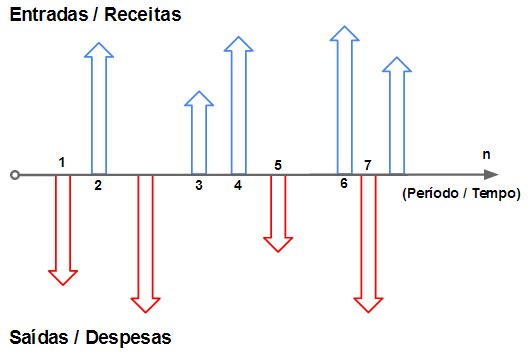
\includegraphics[width=4.16667in,height=\textheight,keepaspectratio]{img/diagrama-fc.png}
\end{center}

\section*{Convenções e Distinções
Essenciais}\label{convenuxe7uxf5es-e-distinuxe7uxf5es-essenciais}
\addcontentsline{toc}{section}{Convenções e Distinções Essenciais}

\markright{Convenções e Distinções Essenciais}

Para aplicar corretamente as ferramentas da matemática financeira,
algumas convenções e distinções são cruciais.

\begin{itemize}
\item
  \textbf{Perspectiva de Caixa vs.~Contabilidade:} Uma distinção
  fundamental deve ser feita entre a base de \textbf{caixa} da análise
  financeira e a base de \textbf{competência} da contabilidade. A
  contabilidade pode reconhecer uma receita ou lucro no momento em que a
  venda é realizada (emissão da nota fiscal), mesmo que o pagamento só
  ocorra meses depois. A matemática financeira, por outro lado, se
  preocupa com o momento em que o \textbf{dinheiro efetivamente entra ou
  sai do caixa}. Isso ocorre porque o dinheiro tem valor no tempo. Um
  lucro de R\$ 20 registrado hoje, mas cujo caixa só será recebido em 90
  dias, não tem o mesmo valor que R\$ 20 em caixa hoje, pois o dinheiro
  imediato poderia ser reinvestido. \emph{Portanto, o fluxo de caixa, e
  não o lucro contábil, é o insumo fundamental para a avaliação
  financeira}.
\item
  \textbf{Alinhamento entre Taxa e Período:} A taxa de juros (\(i\))
  deve sempre ser especificada com uma unidade de tempo (ex: 2\%
  \textbf{ao mês}, 10\% \textbf{ao ano}). Não existe ``taxa de 2\%''.
  Nas fórmulas financeiras, a taxa (\(i\)) e o período (\(n\)) devem
  estar expressos na mesma unidade de tempo. \emph{Se a taxa é mensal, o
  período deve ser medido em meses}.
\item
  \textbf{Forma Unitária nos Cálculos:} Embora as taxas sejam comumente
  discutidas em formato percentual (ex: 12\%), elas devem ser inseridas
  nas equações em sua \textbf{forma unitária (decimal)}. \emph{Uma taxa
  de 12\% ao ano entra na fórmula como 0,12}. Esquecer essa conversão é
  uma fonte comum de erros para iniciantes e deve ser evitado
  rigorosamente.
\end{itemize}

\end{tcolorbox}

\section*{Outros recursos didáticos}\label{outros-recursos-diduxe1ticos}
\addcontentsline{toc}{section}{Outros recursos didáticos}

\markright{Outros recursos didáticos}

Nesta seção, introduzimos os conceitos fundamentais de finanças
corporativas, com foco na relação risco-retorno. Discutimos como as
decisões financeiras são tomadas em um ambiente de incerteza e como o
custo de oportunidade e a taxa de juros influenciam essas decisões. A
compreensão desses princípios é essencial para a boa gestão das finanças
de curto prazo de uma empresa.

Abaixo, você encontrará outros recursos didáticos que objetiva resumir
os conceitos apresentados por aqui:

\begin{quote}
\href{./resources/intro-ppt.html}{\textbf{Slides da Aula}}
\end{quote}

\begin{quote}
\href{./resources/intro-interativo.html}{\textbf{Resumo Interativo}} ➔
\textbf{Resumo do resumo!} 🥱
\end{quote}

\begin{quote}
\href{resources/intro-podcast.mp3}{\textbf{Podcast do Conteúdo}}
\end{quote}

Seu navegador não suporta o elemento de áudio.

\bookmarksetup{startatroot}

\chapter{Capital de Giro}\label{sec-giro}

A administração do capital de giro é uma das áreas mais importantes,
complexas e abrangentes da gestão financeira de uma organização. Ela se
concentra nos recursos de curto prazo da empresa, ou seja, o ativo
circulante e o passivo circulante, e como esses elementos se
inter-relacionam. O objetivo primordial da gestão do capital de giro é
gerar valor para os proprietários e stakeholders.

\section{Capital de Giro (CG) ou Capital Circulante
(CC)}\label{capital-de-giro-cg-ou-capital-circulante-cc}

O Capital Circulante (CC), também conhecido como Capital de Giro (CG), é
a interpretação mais ampla do conceito e corresponde, em sua essência,
ao ativo circulante de uma empresa. Ele representa o valor total dos
recursos necessários para financiar o ciclo operacional diário da
empresa.

As decisões de compra e venda da empresa, assim como suas atividades
operacionais e financeiras, envolvem a administração do capital de giro.
Sua função é garantir a execução adequada das políticas de estocagem,
compra de materiais, produção, venda de produtos/mercadorias e prazo de
recebimento.

A importância e o volume do capital de giro variam em função das
características da empresa (como volume de vendas e sazonalidade), do
desempenho da economia (fatores cíclicos), da tecnologia empregada e da
política de negócios adotada.

\subsection{Capital Circulante Líquido (CCL) ou Capital de Giro Líquido
(CGL)}\label{capital-circulante-luxedquido-ccl-ou-capital-de-giro-luxedquido-cgl}

O Capital Circulante Líquido (CCL), frequentemente chamado de Capital de
Giro Líquido (CGL), é uma das interpretações mais usuais do capital de
giro. Ele representa o valor líquido das aplicações processadas no ativo
circulante da empresa, após a dedução das dívidas de curto prazo.

A forma mais direta de calculá-lo é pela simples diferença entre o Ativo
Circulante (AC) e o Passivo Circulante (PC):

\[CCL = \text{Ativo Circulante} - \text{Passivo Circulante}\]

De uma perspectiva mais rigorosa e conceitual, o Capital Circulante
Líquido (CCL) representa a parcela dos recursos de longo prazo (recursos
permanentes) que é aplicada em itens ativos de curto prazo
(circulantes). Essa interpretação é feita ``de baixo para cima'' no
balanço patrimonial, identificando os valores do passivo de longo prazo
(próprios ou de terceiros) que estão financiando o ativo circulante.
Algebricamente, pode ser obtido pela expressão:

\[
\begin{split}
CCL = & (\text{Passivo Não Circulante} + \text{Patrimônio Líquido}) \\
      & - (\text{Realizável a Longo Prazo} + \text{Ativo Permanente}) = (PNC + PL) - ANC
\end{split}
\]

Ambas as identidades resultam no mesmo valor para o CCL. Para uma
empresa, um CCL positivo indica que parte de suas obrigações de longo
prazo está financiando seu ativo circulante, proporcionando uma folga na
liquidez. Isso significa que a empresa possui mais direitos a receber do
que a pagar no curto prazo. No mundo real, espera-se que essa diferença
seja positiva.

\subsection{Capital de Giro Próprio
(CGP)}\label{capital-de-giro-pruxf3prio-cgp}

O Capital de Giro Próprio (CGP) é um indicador de capital de giro que
representa a parcela de recursos próprios que a empresa tem aplicada em
seu ativo circulante. Ele é comumente obtido pela seguinte expressão:

\[CGP = \text{Patrimônio Líquido (PL)} - \text{Ativo Não Circulante (ANC)}\]

\section{Dinâmica Empresarial: Análise dos Ciclos Operacional e
Financeiro}\label{dinuxe2mica-empresarial-anuxe1lise-dos-ciclos-operacional-e-financeiro}

Entender os ciclos operacionais e financeiros de uma empresa é essencial
para a administração financeira de curto prazo, pois eles revelam a
dinâmica dos fluxos de caixa e a necessidade de financiamento.

\subsection{Ciclo Operacional}\label{ciclo-operacional}

O ciclo operacional é o período que a empresa leva desde a compra de
matéria-prima (ou mercadorias para revenda) até o recebimento das vendas
de seus produtos.

Para uma manufatura, o ciclo operacional pode ser decomposto nas
seguintes fases:

\begin{itemize}
\tightlist
\item
  PME\textsubscript{MP} (Prazo Médio de Estocagem de Matéria-Prima)
\item
  PMF (Prazo Médio de Fabricação)
\item
  PME\textsubscript{PA} (Prazo Médio de Estocagem de Produtos Acabados)
\item
  PMR (Prazo Médio de Recebimento) ou PMC (Prazo Médio de Cobrança)
\end{itemize}

Ciclo Operacional Total (CO) = PME\textsubscript{MP} + PMF +
PME\textsubscript{PA} (ou PME) + PMR (ou PMC)

No entanto, em um comércio essa ``sopa de letrinhas pode ser
simplificada'':

\[CO = PME + PMR\]

\subsection{Ciclo Financeiro (Ciclo de
Caixa)}\label{ciclo-financeiro-ciclo-de-caixa}

O ciclo financeiro (CF), também conhecido como ciclo de caixa (CC),
focaliza as movimentações de caixa, abrangendo o período entre o momento
em que a empresa realiza os pagamentos e o momento em que recebe pelas
vendas.

\[CC = CO - PMP\]

\subsection{Cálculo dos Prazos
Médios}\label{cuxe1lculo-dos-prazos-muxe9dios}

As expressões de cálculo das durações de cada fase operacional,
considerando um empresa comercial, são:

\begin{itemize}
\tightlist
\item
  \textbf{Prazo Médio de Estoques (PME):}
  \[PME = \frac{\text{Estoque Médio}}{\text{Custo das Mercadorias Vendidas Diário}}\]
\item
  \textbf{Prazo Médio de Recebimento (PMR):}
  \[PMR = \frac{\text{Contas a Receber Médias}}{\text{Vendas Líquidas Diárias}}\]
\item
  \textbf{Prazo Médio de Pagamento a Fornecedores (PMP):}
  \[PMP = \frac{\text{Contas a Pagar Médias}}{\text{Custo das Mercadorias Vendidas Diário}}\]
\end{itemize}

\section{Investimento em Capital de
Giro}\label{investimento-em-capital-de-giro}

O investimento em capital de giro é fundamentalmente direcionado à
sustentação da atividade operacional da empresa. As empresas enfrentam
um dilema risco-rentabilidade na definição de suas políticas de
investimento em capital de giro:

\begin{itemize}
\tightlist
\item
  \textbf{Conservadora:} Maiores saldos de caixa, política de crédito
  mais frouxa e maiores estoques. Reduz o risco de liquidez, mas pode
  diminuir a rentabilidade.
\item
  \textbf{Agressiva:} Reduções progressivas nos investimentos em ativos
  circulantes. Eleva o risco da empresa, mas incrementa a rentabilidade.
\item
  \textbf{Média:} Uma abordagem intermediária que busca um equilíbrio
  entre risco e rentabilidade.
\end{itemize}

A determinação do nível ideal de investimento exige um balanço entre os
\textbf{custos de carregamento} (carrying costs) e os \textbf{custos de
falta} (shortage costs).

\section{Financiamento do Capital de
Giro}\label{financiamento-do-capital-de-giro}

As decisões de financiamento buscam a melhor proporção entre capital de
terceiros e capital próprio.

\begin{itemize}
\tightlist
\item
  \textbf{Comportamento das Taxas de Juros a Curto e Longo Prazos}
\end{itemize}

Geralmente, o custo de um crédito a longo prazo é mais caro que o de
curto prazo.

\begin{itemize}
\tightlist
\item
  \textbf{Dilema Risco-Retorno na Composição de Financiamento}
\end{itemize}

Optar por uma maior participação do passivo circulante pode aumentar os
resultados líquidos (menores custos), mas também aumenta o risco
financeiro.

\subsection{Abordagens para o Financiamento do Capital de
Giro}\label{abordagens-para-o-financiamento-do-capital-de-giro}

O capital de giro é classificado como \textbf{permanente} (ou fixo) e
\textbf{sazonal} (ou variável). As principais abordagens de
financiamento são:

\begin{itemize}
\tightlist
\item
  \textbf{Abordagem pelo Equilíbrio Financeiro Tradicional:} Ativo
  permanente e capital de giro permanente financiados por recursos de
  longo prazo; necessidades sazonais de capital de giro cobertas por
  exigibilidades de curto prazo.
\item
  \textbf{Abordagem de Risco Mínimo (Conservadora):} A empresa é
  totalmente financiada por recursos permanentes (longo prazo).
\item
  \textbf{Abordagem Restritiva (Agressiva):} Usa financiamento de longo
  prazo apenas para as necessidades permanentes de ativos imobilizados e
  capital de giro.
\end{itemize}

\subsection{Fontes de Financiamento de Curto
Prazo}\label{fontes-de-financiamento-de-curto-prazo}

As fontes podem ser \textbf{espontâneas} (contas a pagar a fornecedores,
despesas a pagar) ou \textbf{negociadas} (empréstimos bancários,
commercial papers, empréstimos com garantia).

\section{Necessidade de Investimento em Capital de Giro
(NIG)}\label{necessidade-de-investimento-em-capital-de-giro-nig}

A Necessidade de Investimento em Giro (NIG) reflete o volume líquido de
recursos demandado pelo ciclo operacional da empresa.

\subsection{Distinção entre Componentes da
NIG}\label{distinuxe7uxe3o-entre-componentes-da-nig}

A Necessidade de Capital de Giro (NCG) é a diferença entre os usos
operacionais (Ativo Circulante Operacional - ACO) e as fontes
operacionais (Passivo Circulante Operacional - PCO):

\[NCG = ACO - PCO\]

\subsection{Saldo de Tesouraria e o Efeito
Tesoura}\label{saldo-de-tesouraria-e-o-efeito-tesoura}

A diferença entre a Necessidade de Capital de Giro (NCG) e o Capital de
Giro (CDG) é conhecida como Saldo de Tesouraria (ST):

\[ST = CDG - NCG\]

O ``efeito tesoura'' é uma situação crítica que ocorre quando o índice
NCG/Vendas cresce de forma mais rápida do que o índice CDG/Vendas,
levando a uma necessidade de aportes financeiros crescente.

\section*{Outros recursos
didáticos}\label{outros-recursos-diduxe1ticos-1}
\addcontentsline{toc}{section}{Outros recursos didáticos}

\markright{Outros recursos didáticos}

Nesta seção, falamos um pouco sobre os principais indicadores de
eficiência da gestão de curto prazo, tal como ciclos (operacional e de
caixa), prazos médios e investimento/financiamento do capital de giro.

Abaixo, você encontrará outros recursos didáticos que objetiva resumir
os conceitos apresentados por aqui:

\begin{quote}
\href{./resources/giro-ppt.html}{\textbf{Slides da Aula}}
\end{quote}

\begin{quote}
\href{./resources/giro-interativo.html}{\textbf{Resumo Interativo}} ➔
\textbf{Resumo do resumo!} 🥱
\end{quote}

\begin{quote}
\href{resources/giro-podcast.mp3}{\textbf{Podcast do Conteúdo}}
\end{quote}

Seu navegador não suporta o elemento de áudio.

\bookmarksetup{startatroot}

\chapter{Administração do Caixa}\label{sec-caixa}

A administração de caixa é uma função central da gestão financeira de
curto prazo, cujo objetivo é otimizar a liquidez da empresa, garantindo
que ela possa honrar seus compromissos e, ao mesmo tempo, maximizar o
retorno sobre os recursos monetários que, de outra forma, estariam
ociosos. A gestão eficaz do caixa reside no equilíbrio entre o custo de
oportunidade de manter saldos elevados e o risco de insolvência
decorrente de saldos insuficientes.

Ao priorizar os tópicos de Administração de Caixa que, resumidamente,
discorremos abaixo, temos como objetivo garantir que os alunos recebam
um conhecimento detalhado e direcionado sobre as técnicas e modelos
específicos da gestão de caixa de curto prazo, sem que o conteúdo seja
diluído por tópicos mais amplos que são exaustivamente tratados em
outras partes do curso ou em outras disciplinas, por exemplo, a
disciplina de Planejamento Financeiro e Orçamento Empresarial trata do
confecção do fluxo de caixa.

Isso permite uma abordagem mais eficaz e concisa para o segmento de
curto prazo, conforme a estrutura e os objetivos da ementa oficial, que
está mais alinhada com o livro-texto do Assaf Neto (2014).

\section{Razões para a Manutenção de
Caixa}\label{razuxf5es-para-a-manutenuxe7uxe3o-de-caixa}

A teoria da preferência pela liquidez de John Maynard Keynes fornece a
base teórica para entender por que as empresas demandam e mantêm saldos
de caixa. Esses motivos são:

\begin{itemize}
\item
  \textbf{Motivo Transação (ou Negócio):} Esta é a razão mais
  fundamental para a manutenção de caixa. Surge da necessidade de cobrir
  os desembolsos decorrentes das operações normais e previsíveis do
  negócio, como pagamento de fornecedores, salários, impostos e outras
  despesas correntes. A necessidade de caixa para transações é
  diretamente influenciada pela falta de sincronia perfeita entre os
  fluxos de entrada (recebimentos) e saída (pagamentos) de recursos.
\item
  \textbf{Motivo Precaução:} Este motivo está associado à incerteza
  inerente ao ambiente de negócios. Os fluxos de caixa reais raramente
  correspondem exatamente aos orçados. Portanto, as empresas mantêm um
  saldo de caixa de precaução como uma reserva de segurança (um
  ``colchão'' de liquidez) para se proteger contra flutuações
  inesperadas e adversas, como um atraso no recebimento de um cliente
  importante ou um aumento súbito no custo de matérias-primas. Esse
  saldo garante a capacidade de pagamento mesmo em cenários
  desfavoráveis.
\item
  \textbf{Motivo Especulação:} Refere-se à manutenção de caixa para
  capitalizar oportunidades de mercado imprevistas e vantajosas. Uma
  empresa com liquidez pode, por exemplo, adquirir um grande lote de
  matéria-prima com um desconto significativo, realizar uma aquisição
  estratégica de um concorrente em dificuldades ou aproveitar outras
  oportunidades de investimento que exijam desembolso imediato.
\end{itemize}

\section{Ciclo de Caixa e Estratégias de
Controle}\label{ciclo-de-caixa-e-estratuxe9gias-de-controle}

O Ciclo de Caixa (CC), também conhecido como Ciclo Financeiro (CF), é a
métrica temporal que quantifica a necessidade de financiamento do
capital de giro. Ele mede o número de dias entre o pagamento aos
fornecedores pela matéria-prima e o recebimento efetivo do dinheiro pela
venda do produto acabado. O objetivo estratégico do gestor financeiro é
minimizar a duração deste ciclo, pois um ciclo mais curto implica uma
menor necessidade de recursos para sustentar as operações e,
consequentemente, um menor custo de capital.

O controle e a otimização do saldo de caixa podem ser realizados por
meio de duas categorias de medidas:

\begin{itemize}
\item
  \textbf{Medidas de Competência Exclusiva do Caixa:} Ações táticas
  focadas diretamente na aceleração das entradas e no gerenciamento das
  saídas. Incluem a dinamização dos processos de cobrança, a redução do
  tempo entre a venda e a emissão da fatura, e a busca por uma
  sincronização ótima entre as datas de recebimento e pagamento.
\item
  \textbf{Medidas de Política Ampla:} Ações estratégicas que envolvem
  outras áreas da empresa. Incluem a revisão da política de crédito
  (prazos e condições oferecidos aos clientes), a otimização dos níveis
  de estoque para reduzir o capital imobilizado e a criação de uma
  política de aplicação dos saldos de caixa temporariamente ociosos em
  títulos negociáveis de alta liquidez.
\end{itemize}

O Saldo Mínimo de Caixa é o nível de caixa que permite à empresa cobrir
seus desembolsos programados e manter uma reserva de segurança. Um
modelo determinístico para seu cálculo é:

\[\text{Saldo Mínimo de Caixa} = \frac{\text{Desembolsos Totais de Caixa Esperados no Período}}{\text{Giro de Caixa no Período (GC)}}\]

Onde \(GC\) pode ser calculado pela divisão 360 dias pelo \(CC\) (em
dias).

Este modelo, contudo, possui limitações por não incorporar a incerteza.
Para torná-lo mais realista, ajustes são necessários, como a análise de
horizontes de tempo mais curtos e a consideração da sazonalidade das
operações.

\section{Modelos Quantitativos de Administração de
Caixa}\label{modelos-quantitativos-de-administrauxe7uxe3o-de-caixa}

Para refinar a decisão sobre o nível ótimo de caixa, modelos
quantitativos foram desenvolvidos. Eles buscam minimizar os custos
totais associados à gestão da liquidez, que são, fundamentalmente, o
custo de oportunidade e o custo de transação.

\subsection{Modelo de Lote Econômico
(Baumol)}\label{modelo-de-lote-econuxf4mico-baumol}

Desenvolvido por William Baumol, este modelo determinístico trata o
caixa como um estoque e aplica a lógica do lote econômico de compras.
Ele busca o saldo de caixa ótimo (C) que minimiza a soma de dois custos
conflitantes:

\textbf{Custo de Oportunidade (Custo de Manutenção):} Representa os
juros que a empresa deixa de ganhar por manter recursos em caixa em vez
de investi-los em títulos negociáveis. É calculado como:

\[\text{Custo de Manutenção (CM)} = i \times \frac{C}{2}\]

Onde \(i\) é a taxa de juros dos títulos e \(\frac{C}{2}\) é o saldo
médio de caixa (\(\bar{C}\)).

\textbf{Custo de Transação (Custo de Obtenção):} Representa os custos
fixos incorridos cada vez que a empresa converte títulos em caixa (ex:
taxas de corretagem). É calculado como:

\[\text{Custo de Obtenção (CO)} = b \times \frac{T}{C}\]

Onde \(b\) é o custo fixo por transação, \(T\) é a necessidade total de
caixa no período e \(\frac{T}{C}\) é o número de transações (\(N\)). Ao
somarmos \(CM\) + \(CO\), temos:

\[CT = \left( b \times \frac{T}{C} \right) + \left( i \times \frac{C}{2} \right)\]

Igualando \(CT\) a zero e resolvendo para \(C\) obtemos a fórmula do
Saldo Ótimo (\(C^*\)) de Baumol:

\[C^* = \sqrt{\frac{2 \times b \times T}{i}}\]

A principal limitação do modelo de Baumol é sua natureza determinística:
ele assume que os fluxos de caixa são perfeitamente previsíveis e que
seu uso é constante ao longo do tempo, o que raramente ocorre na
prática.

\subsection{Modelo de Miller e Orr}\label{modelo-de-miller-e-orr}

Este é um modelo estocástico (probabilístico), mais sofisticado e
realista, pois foi projetado para lidar com a incerteza dos fluxos de
caixa diários. Ele assume que as variações líquidas diárias no caixa são
aleatórias. O modelo funciona estabelecendo limites de controle para o
saldo de caixa:

\textbf{Limite Superior (h):} Quando o saldo de caixa atinge este ponto,
a empresa utiliza o excedente para comprar títulos negociáveis,
retornando o saldo de caixa a um nível predefinido (o ``ponto de
retorno'', z).

\textbf{Limite Inferior (L):} Geralmente definido como zero ou um saldo
mínimo de segurança. Quando o caixa atinge este ponto, a empresa vende
títulos para obter caixa e elevar o saldo novamente até o ponto de
retorno (z).

O objetivo do modelo é minimizar os custos totais esperados
(oportunidade e transação). O ponto de retorno ótimo (z), que é a
variável chave do modelo, é calculado pela seguinte fórmula:

\[z = \sqrt[3]{\frac{3 \times b \times \sigma^2}{4 \times i}} + L\]

Onde: - \(z\) = Ponto de retorno ótimo; \(b\) = Custo fixo por transação
com títulos; \(\sigma^2\) = Variância dos fluxos líquidos diários de
caixa; \(i\) = Taxa de juros diária dos títulos negociáveis; \(L\) =
Limite Inferior

A banda superior do caixa, na assunção de um saldo mínimo de segurança
(L), pode ser calculado como:

\[h = 3z - 2L\]

\subsection{O Dilema da Gestão de Caixa em Cenários
Inflacionários}\label{o-dilema-da-gestuxe3o-de-caixa-em-cenuxe1rios-inflacionuxe1rios}

A inflação impõe um desafio adicional e significativo à administração de
caixa. A principal consequência é a perda do poder de compra da moeda
mantida em caixa. Isso cria um dilema com duas forças conflitantes:

\begin{itemize}
\item
  Por um lado, a inflação eleva os custos operacionais, o que aumenta a
  necessidade de investimento nominal em capital de giro para que a
  empresa consiga manter o mesmo nível de atividade real.
\item
  Por outro lado, para se proteger da depreciação monetária, a
  estratégia racional é manter o saldo de caixa o mais baixo possível,
  aplicando quaisquer recursos excedentes em títulos negociáveis que
  ofereçam proteção contra a inflação (por exemplo, atrelados a um
  índice de preços).
\end{itemize}

Em conjunturas inflacionárias, as políticas de minimização dos saldos de
caixa tornam-se, portanto, ainda mais cruciais para a preservação do
valor da empresa.

\section*{Outros recursos
didáticos}\label{outros-recursos-diduxe1ticos-2}
\addcontentsline{toc}{section}{Outros recursos didáticos}

\markright{Outros recursos didáticos}

Nesta seção, falamos sobre a gestão do caixa e apresentamos os
principais conceitos e modelos utilizados, como o modelo de Baumol e o
modelo de Miller e Orr. Esses modelos ajudam a determinar o saldo ótimo
de caixa, equilibrando os custos de oportunidade e transação, além de
considerar a incerteza dos fluxos de caixa diários. Também discutimos a
importância do ciclo de caixa e as estratégias para otimizar a liquidez
da empresa. Por fim, abordamos o dilema da gestão de caixa em cenários
inflacionários, destacando a necessidade de manter saldos adequados para
preservar o poder de compra.

Abaixo, você encontrará outros recursos didáticos que objetiva resumir
os conceitos apresentados por aqui:

\begin{quote}
\href{./resources/caixa-ppt.html}{\textbf{Slides da Aula}}
\end{quote}

\begin{quote}
\href{./resources/caixa-interativo.html}{\textbf{Resumo Interativo}} ➔
\textbf{Resumo do resumo!} 🥱
\end{quote}

\begin{quote}
\href{resources/caixa-podcast.mp3}{\textbf{Podcast do Conteúdo}}
\end{quote}

Seu navegador não suporta o elemento de áudio.

\bookmarksetup{startatroot}

\chapter{Administração de Recebíveis}\label{sec-credito}

\bookmarksetup{startatroot}

\chapter{Administração de Estoques}\label{sec-estoque}

A administração de estoques é uma área crítica da gestão financeira. Os
estoques, por natureza, são ativos de baixa liquidez que imobilizam um
volume significativo de capital. Uma gestão ineficiente pode comprometer
tanto a rentabilidade, ao inflar os custos de carregamento e o capital
empatado, quanto a liquidez, ao drenar recursos que poderiam ser
alocados em outras necessidades de curto prazo.

O desafio central reside em um equilíbrio delicado:

\begin{itemize}
\item
  \textbf{Minimização do Investimento}: Manter os níveis de estoque os
  mais baixos possíveis para otimizar a rotação, reduzir custos de
  armazenagem, seguro, obsolescência e, fundamentalmente, liberar caixa.
\item
  \textbf{Maximização do Nível de Serviço}: Garantir que não haja
  rupturas no processo de produção ou vendas, o que poderia levar à
  perda de clientes, desgaste da imagem da marca e custos de
  oportunidade irrecuperáveis.
\end{itemize}

\section{Custos Relevantes na Gestão de
Estoques}\label{custos-relevantes-na-gestuxe3o-de-estoques}

As decisões sobre o nível ótimo de estoques envolvem a análise de dois
custos destoantes:

\begin{enumerate}
\def\labelenumi{\arabic{enumi}.}
\tightlist
\item
  \textbf{Custos de Manutenção ou Carregamento:} Custos para manter o
  estoque, como custo de capital, armazenagem, seguros e perdas.
  Aumentam com o volume estocado.
\item
  \textbf{Custos de Pedido (Compra) ou Preparação:} Custos para adquirir
  um novo lote, como processamento, frete e recebimento. Diminuem à
  medida que o tamanho dos lotes aumenta (menos pedidos são feitos).
\end{enumerate}

Um dos objetivos da gestão financeira de estoque é operacionar modelos
de otimização para encontrar o ponto em que a soma desses dois grupos de
custos seja minimizada. No entanto, antes de aplicar modelos de
otimização complexos, é fundamental direcionar os esforços de gestão.

\section{Controle Seletivo: A Curva
ABC}\label{controle-seletivo-a-curva-abc}

Nem todos os itens de estoque possuem a mesma importância financeira.
Para otimizar os esforços de gestão, os estoques são classificados pela
sua importância financeira usando a \textbf{Curva ABC}, uma aplicação do
\textbf{Princípio de Pareto}.

O Princípio de Pareto, ou \textbf{regra 80/20}, postula que, para muitos
eventos, aproximadamente \emph{80\% dos efeitos vêm de 20\% das causas}.
Aplicado aos estoques, isso significa que uma pequena porcentagem dos
itens em inventário (os 20\%) tende a ser responsável por uma grande
porcentagem do valor total de consumo ou venda (os 80\%).

\begin{itemize}
\tightlist
\item
  \textbf{Classe A:} Poucos itens (ex: 20\%) que representam a maior
  parte do valor (ex: 80\%). Exigem controle rigoroso e modelos de
  otimização.
\item
  \textbf{Classe B:} Itens de importância intermediária.
\item
  \textbf{Classe C:} Muitos itens (ex: 50\%) de baixo valor individual.
  Admitem controles mais simples.
\end{itemize}

A Curva ABC direciona a atenção gerencial para onde ela é mais crítica,
garantindo que os itens mais valiosos (Classe A) sejam gerenciados com a
máxima eficiência.

\subsection{Simulador da Curva ABC}\label{simulador-da-curva-abc}

Abaixo você pode visualizar a metodologia de cálculo da Curva ABC em
operação, ou você pode expandir essa versão interativa do simulador da
Curva ABC clicando no link:

\begin{quote}
\href{./resources/curvaABC.html}{\textbf{Simulador da Curva ABC}}
\end{quote}

\section{Decisões de Compra}\label{decisuxf5es-de-compra}

A decisão de quando e como pagar por um lote de estoque é um problema
clássico de valor do dinheiro no tempo. A metodologia tradicionalmente
apresentada em finanças corporativas pode ser perfeitamente reenquadrada
e aprofundada pela ótica da \textbf{Equivalência de Capitais}.

A análise compara diferentes propostas de compra (ex: à vista vs.~a
prazo) tratando cada uma na linha do tempo (diagrama de caixa). Nesse
caso, a variável central é o período, que em nosso contexto, pode ser
entendido pelo \textbf{Ciclo de Caixa (CC)}.

\[
CC~(\text{dias}) = PME + PMR - PMP
\]

Onde: \(PME\): Prazo Médio de Estocagem, \(PMR\): Prazo Médio de
Recebimento e \(PMP\): Prazo Médio de Pagamento

O sinal do CC define quem financia a operação e qual taxa de juros
(custo de oportunidade) utilizar.

\subsection{Cenário 1: Ciclo de Caixa
Positivo}\label{cenuxe1rio-1-ciclo-de-caixa-positivo}

A empresa paga o fornecedor antes de receber do cliente, precisando
\textbf{financiar a operação}. A taxa relevante é o \textbf{Custo de
Captação (}\(k_c\)).

O \textbf{Diagrama de Fluxo de Caixa} abaixo ilustra a saída de caixa
(Custo) ocorrendo antes da entrada (Venda):

\subsection{Cenário 2: Ciclo de Caixa
Negativo}\label{cenuxe1rio-2-ciclo-de-caixa-negativo}

A empresa recebe do cliente antes de pagar o fornecedor, sendo
\textbf{financiada pelo fornecedor}. A taxa relevante é a \textbf{Taxa
de Aplicação (}\(k_a\)).

Note como a ordem dos eventos se inverte no \textbf{Diagrama de Fluxo de
Caixa}: a entrada (Venda) agora ocorre antes da saída (Custo).

\subsection{Formulação Geral}\label{formulauxe7uxe3o-geral}

O resultado da operação (\(R\)) é calculado em uma data focal comum
(\(t_r\), data de recebimento), usando a taxa apropriada:

\[
\text{R}_{t_r} = \text{PV} - \left[ \text{CMV} \times (1 + i)^{\frac{CC}{30}} \right]
\]

Onde \(i = k_c\) se \(CC > 0\), e \(i = k_a\) se \(CC < 0\). \(PV\) é
preço de venda que já se encontra na data \(t_r\) e \(CMV\) é o custo da
mercadoria vendida capitalizado (se \(CC > 0\)) ou descapitalizado (se
\(CC < 0\)) para a data \(t_r\).

\subsection{Simulador Decisões de
Compra}\label{simulador-decisuxf5es-de-compra}

Abaixo você pode visualizar a formulação geral para tomada de decisões
de compra de estoque em operação, ou você pode expandir essa versão
interativa do Simulador de Decisões de Compra clicando no link:

\begin{quote}
\href{./resources/decisoes-compra.html}{\textbf{Simulador Decisões de
Compra}}
\end{quote}

\section{O Modelo do Lote Econômico de Compra
(LEC)}\label{o-modelo-do-lote-econuxf4mico-de-compra-lec}

O LEC é um modelo de otimização que determina a quantidade ideal a ser
comprada em cada pedido para minimizar os custos totais de gestão de
estoques. Ele encontra o ponto onde os custos de manutenção se igualam
aos custos de pedido.

A fórmula do LEC é:

\[
LEC = \sqrt{\frac{2 \times D \times C_p}{C_m}}
\]

Onde: \(D\): Demanda total no período, \(C_p\): Custo de cada pedido e
\(C_m\): Custo de manutenção por unidade.

Enquanto a análise anterior foca em decisões de compra pontuais, o LEC
busca responder a uma pergunta recorrente: \emph{Qual a quantidade ideal
a ser pedida em cada lote para minimizar os custos totais de gestão de
estoques ao longo de um período?}

\subsection{Derivação do LEC}\label{derivauxe7uxe3o-do-lec}

O LEC parte das premissas de demanda constante e conhecida, preço de
compra constante, prazo de entrega (lead time) constante e conhecido e
custo de manutenção e de pedido constante e conhecido, ou seja, o LEC é
um modelo em condicões de certeza ou certa estabilidade preditiva.

O modelo se baseia em um trade-off:

\begin{itemize}
\tightlist
\item
  Pedir lotes grandes diminui o custo anual de pedidos (CP), mas aumenta
  o custo anual de manutenção (CM).
\end{itemize}

\[
\text{CP} = C_p \times \frac{D}{Q}
\] Onde: \(Q\) representa a quantidade de cada pedido (em unidades) e
\emph{D/Q} representa o número total de pedidos (N):

\[
\text{N} = \frac{D}{Q}
\]

\begin{itemize}
\tightlist
\item
  Pedir lotes pequenos diminui o custo anual de manutenção (CM), mas
  aumenta o custo anual de pedidos (CP).
\end{itemize}

\[
\text{CM} = C_m \times \frac{Q}{2}
\]

\emph{Q/2} representa o estoque médio (EM).

O Custo Total (CT) é a soma dos dois custos: CP + CM

\[
\text{CT} = \left(C_p \times \frac{D}{Q}\right) + \left(C_m \times \frac{Q}{2}\right)
\] Igualando CT a zero, ou de outra forma, CP = CM, temos:

\[
C_p \times \frac{D}{Q} = C_m \times \frac{Q}{2}
\]

Multiplicando ambos os lados por Q:

\[
C_p \times \frac{D}{Q} \times Q = C_m \times \frac{Q}{2} \times Q
\]

\[
C_p \times D = C_m \times \frac{Q^2}{2}
\]

Multiplicando ambos os lados por 2:

\[
2 \times C_p \times D = C_m \times Q^2
\]

Isolando \(Q^2\):

\[
Q^2 = \frac{2 \times C_p \times D}{C_m}
\]

Extraindo a raiz quadrada para obter o LEC (\(Q^*\)), temos:

\[
Q^* = \sqrt{\frac{2 \times C_p \times D}{C_m}}
\]

\subsection{Simulador LEC}\label{simulador-lec}

Abaixo você pode visualizar o LEC em operação, ou você pode expandir
esse o Simulador do LEC no link:

\begin{quote}
\href{./resources/lec.html}{\textbf{Simulador LEC}}
\end{quote}

\bookmarksetup{startatroot}

\chapter{Projetos em Grupo}\label{sec-aval}

O objetivo desse módulo final é criar a oportunidade de o aluno
aprofundar (um pouco mais!) nas bases fundamentais das finanças. Em
cursos de graduação em negócios (Economia, Administração e Contábeis)
temos outras disciplinas de finanças, que o aluno aprende sobre teorias
importantes, tal como Estrutura de Capital em Finanças Corporativas (II)
de Longo Prazo, no entanto, algumas relevantes teorias são relegadas
como optativas ou de carácter secundário, pelo menos, na graduação. A
intenção aqui é que o aluno tenha um primeiro contato sobre esses
fundamentos.

Abaixo eu apresento um resumo dos capítulos 1 e 2 do Assaf Neto (2014),
que faz parte de nossa ementa oficial, principalmente, o conteúdo de
Governança Corporativa (Propriedade e administração, e Conflitos de
Agência), no entanto, nos projetos em grupos, além da Governança
Corporativa, discutiremos a Teoria da Utilidade, Hipóteses de Mercados
Eficientes, Teoria do Portfólio, Teoria de Precificação por Arbitragem e
Finanças Comportamentais.

\section{O Objetivo da Empresa e da Administração
Financeira}\label{o-objetivo-da-empresa-e-da-administrauxe7uxe3o-financeira}

A administração financeira é a área que se ocupa da gestão dos recursos
de uma organização, com o objetivo de criar valor. Para entender suas
funções, é primordial definir o objetivo central da empresa.

\subsection{O Objetivo da Empresa}\label{o-objetivo-da-empresa}

Embora a maximização do lucro seja uma resposta intuitiva, ela é
insuficiente como objetivo principal da administração financeira por
três razões críticas:

\begin{enumerate}
\def\labelenumi{\arabic{enumi}.}
\tightlist
\item
  \textbf{Ignora o Tempo:} A maximização do lucro não especifica o
  horizonte temporal. Uma empresa pode aumentar os lucros de curto prazo
  ao cortar custos essenciais, como manutenção ou pesquisa, mas essa
  atitude pode destruir valor no longo prazo.
\item
  \textbf{Ignora o Fluxo de Caixa:} O lucro contábil não é sinônimo de
  dinheiro em caixa. Uma empresa pode registrar lucro em suas
  demonstrações e, ainda assim, não ter liquidez para honrar seus
  compromissos, o que pode levá-la à falência.
\item
  \textbf{Ignora o Risco:} A meta de maximizar o lucro não considera o
  risco associado à geração desses lucros. Dois projetos podem ter o
  mesmo lucro esperado, mas um pode ser significativamente mais
  arriscado que o outro.
\end{enumerate}

O objetivo mais apropriado e abrangente da administração financeira é,
portanto, \textbf{maximizar a riqueza dos acionistas}, que é mensurada
pelo valor de mercado de suas ações. O preço da ação reflete as
expectativas do mercado sobre os fluxos de caixa futuros da empresa,
devidamente ajustados pelo risco e pelo tempo.

\subsection{Visão dos Shareholders
vs.~Stakeholders}\label{visuxe3o-dos-shareholders-vs.-stakeholders}

No centro da discussão sobre o objetivo da empresa está a distinção
entre dois grupos:

\begin{itemize}
\tightlist
\item
  \textbf{Shareholders (Acionistas):} São os proprietários da empresa. A
  maximização de sua riqueza é o foco principal da gestão financeira,
  especialmente em modelos de mercado anglo-saxônicos (EUA, Reino
  Unido). Os acionistas são considerados os ``proprietários residuais'',
  pois só recebem seu retorno após todos os outros compromissos da
  empresa serem pagos.
\item
  \textbf{Stakeholders (Partes Interessadas):} É um grupo mais amplo que
  inclui qualquer indivíduo ou entidade com interesse na empresa, como
  funcionários, clientes, fornecedores, credores e a comunidade.
\end{itemize}

Embora o objetivo primário seja a maximização do valor para o acionista,
uma gestão eficaz reconhece que a criação de valor no longo prazo
depende de um relacionamento saudável com todos os stakeholders. Ignorar
os interesses dos funcionários ou clientes, por exemplo, inevitavelmente
prejudicaria a reputação e os resultados da empresa, destruindo o valor
para o acionista.

\subsection{As Decisões Fundamentais: Investimento e
Financiamento}\label{as-decisuxf5es-fundamentais-investimento-e-financiamento}

A atividade do administrador financeiro pode ser resumida em duas
decisões centrais, que se refletem diretamente no balanço patrimonial da
empresa:

\begin{enumerate}
\def\labelenumi{\arabic{enumi}.}
\tightlist
\item
  \textbf{Decisão de Investimento (Orçamento de Capital):} Refere-se à
  alocação de recursos em ativos de longo prazo. Envolve decidir em
  quais projetos investir, como a construção de uma nova fábrica ou o
  lançamento de um produto. Essas decisões determinam a composição do
  lado esquerdo do balanço (Ativos) e são consideradas as mais
  importantes para a criação de valor.
\item
  \textbf{Decisão de Financiamento (Estrutura de Capital):} Refere-se à
  forma como a empresa obterá os fundos necessários para seus
  investimentos. Envolve a escolha entre capital de terceiros (dívida) e
  capital próprio (ações). Essas decisões moldam o lado direito do
  balanço (Passivo e Patrimônio Líquido).
\end{enumerate}

\subsection{Gestão de Curto e Longo Prazo e o Foco no Fluxo de
Caixa}\label{gestuxe3o-de-curto-e-longo-prazo-e-o-foco-no-fluxo-de-caixa}

As decisões financeiras também se dividem pelo horizonte de tempo:

\begin{itemize}
\tightlist
\item
  \textbf{Gestão de Longo Prazo:} Envolve as decisões de investimento e
  financiamento mencionadas acima, que definem o futuro estratégico da
  empresa.
\item
  \textbf{Gestão de Curto Prazo:} Foca na administração do capital de
  giro (ativos e passivos circulantes), garantindo que a empresa tenha
  liquidez para suas operações diárias.
\end{itemize}

Um princípio fundamental que norteia todas essas decisões é o
\textbf{foco no fluxo de caixa}. A contabilidade opera sob o regime de
competência, registrando receitas quando a venda é feita, e não quando o
dinheiro é recebido. Finanças, por outro lado, operam sob o regime de
caixa, preocupando-se com as entradas e saídas efetivas de dinheiro. Uma
empresa pode ser lucrativa do ponto de vista contábil, mas insolvente se
não gerar caixa suficiente para pagar suas obrigações.

\section{Governança Corporativa}\label{governanuxe7a-corporativa}

Governança corporativa é o sistema de regras, práticas e processos pelo
qual uma empresa é dirigida e controlada. Sua principal função é alinhar
os interesses dos gestores com os dos acionistas, mitigando os conflitos
que surgem da separação entre propriedade e gestão.

\subsection{O Conflito de Agência}\label{o-conflito-de-aguxeancia}

O problema de agência surge quando há um conflito de interesses entre o
\textbf{principal} (os acionistas) e o \textbf{agente} (os
administradores contratados para agir em nome dos acionistas). Os
gestores podem, por exemplo, priorizar a segurança de seus empregos ou
benefícios pessoais em detrimento de projetos arriscados que poderiam
maximizar o valor para os acionistas. Os custos decorrentes desse
desalinhamento são chamados de \textbf{custos de agência}.

\subsection{Conflitos de Agência: Diferenças entre Brasil e
EUA}\label{conflitos-de-aguxeancia-diferenuxe7as-entre-brasil-e-eua}

A natureza do principal conflito de agência varia conforme a estrutura
de propriedade do capital, que é notavelmente diferente entre o Brasil e
mercados como os EUA e o Reino Unido:

\begin{itemize}
\tightlist
\item
  \textbf{Nos EUA e Reino Unido,} o capital das grandes empresas é
  tipicamente \textbf{pulverizado}, sem um acionista controlador claro.
  Nesse cenário, o principal conflito de agência ocorre entre
  \textbf{gestores profissionais e os acionistas dispersos}. A
  preocupação central da governança é garantir que os executivos atuem
  no melhor interesse dos proprietários.
\item
  \textbf{No Brasil e na Europa Continental,} a estrutura de propriedade
  é caracterizada pela \textbf{alta concentração de capital}, onde um
  único acionista ou um pequeno bloco de acionistas detém o controle da
  empresa. O principal conflito, portanto, ocorre entre os
  \textbf{acionistas controladores e os acionistas minoritários}. A
  governança busca proteger os minoritários de decisões que possam
  beneficiar desproporcionalmente os controladores.
\end{itemize}

\subsection{Mecanismos de Governança}\label{mecanismos-de-governanuxe7a}

Para mitigar os problemas de agência, as empresas utilizam diversos
mecanismos de governança:

\begin{itemize}
\tightlist
\item
  \textbf{Conselho de Administração:} Eleito pelos acionistas para
  supervisionar a gestão e tomar decisões estratégicas. A presença de
  conselheiros independentes é crucial para um monitoramento eficaz.
\item
  \textbf{Remuneração dos Executivos:} Planos de incentivo, como opções
  de ações e bônus atrelados ao desempenho, que alinham a riqueza dos
  gestores à dos acionistas.
\item
  \textbf{Monitoramento Externo:} Auditorias independentes, analistas de
  mercado e grandes investidores institucionais que fiscalizam as ações
  da empresa.
\item
  \textbf{Ameaça de Aquisição (Takeover):} Empresas mal administradas
  podem se tornar alvos de aquisição, o que pressiona a gestão a
  melhorar o desempenho para evitar ser substituída.
\end{itemize}

\section{Importantes Teorias de
Finanças}\label{importantes-teorias-de-finanuxe7as}

A moderna teoria financeira é sustentada por diversos pilares teóricos
que buscam explicar o comportamento dos mercados e dos investidores.

\begin{itemize}
\tightlist
\item
  \textbf{Teoria da Utilidade:} Proposta por Bernoulli, esta teoria
  postula que os investidores não buscam maximizar o retorno em si, mas
  a ``utilidade'' ou satisfação que a riqueza proporciona. Isso explica
  por que indivíduos têm diferentes perfis de risco (aversão,
  neutralidade ou propensão ao risco), pois a utilidade marginal da
  riqueza é decrescente para a maioria das pessoas.
\item
  \textbf{Hipótese dos Mercados Eficientes:} Desenvolvida por Eugene
  Fama, esta teoria afirma que os preços dos ativos em um mercado
  eficiente refletem instantaneamente toda a informação disponível. Uma
  consequência direta é que se torna extremamente difícil obter retornos
  anormais (ou ``bater o mercado'') de forma consistente, pois não
  haveria ativos sub ou sobreavaliados.
\item
  \textbf{Teoria do Portfólio:} Formulada por Harry Markowitz, esta
  teoria revolucionou a gestão de investimentos ao demonstrar que o
  risco de um ativo não deve ser avaliado isoladamente, mas por sua
  contribuição ao risco total de uma carteira diversificada. A
  diversificação permite reduzir o risco não-sistemático sem
  necessariamente sacrificar o retorno esperado.
\item
  \textbf{Teoria de Precificação por Arbitragem (APT):} Proposta por
  Stephen Ross, a APT é um modelo de precificação de ativos que,
  diferentemente do CAPM (que usa um único fator de risco, o mercado),
  sugere que o retorno de um ativo é uma função linear de múltiplos
  fatores de risco macroeconômicos, como inflação, produção industrial,
  entre outros.
\item
  \textbf{Finanças Comportamentais:} Este campo de estudo, impulsionado
  por psicólogos como Daniel Kahneman e Amos Tversky, desafia o
  pressuposto da racionalidade total dos investidores. Ele investiga
  como vieses cognitivos e emocionais (como excesso de confiança,
  aversão à perda e comportamento de manada) afetam as decisões
  financeiras e podem levar a anomalias e ineficiências nos mercados.
\end{itemize}

\section*{Outros recursos
didáticos}\label{outros-recursos-diduxe1ticos-3}
\addcontentsline{toc}{section}{Outros recursos didáticos}

\markright{Outros recursos didáticos}

Nesta seção, falamos um pouco sobre o objetivo da empresa, os conflitos
de interesse que podem existir na perseguição desses objetivos
(Governança Corporativa) e apresentamos algumas teorias basilares que
nos ajudam a entender as finanças. A introdução desses princípios é
importante para vocês continuarem a busca.

Abaixo, você encontrará outros recursos didáticos que objetiva resumir
os conceitos apresentados por aqui:

\begin{quote}
\href{./resources/teorias-ppt.html}{\textbf{Slides da Aula}}
\end{quote}

\begin{quote}
\href{./resources/teorias-interativo.html}{\textbf{Resumo Interativo}} ➔
\textbf{Resumo do resumo!} 🥱
\end{quote}

\begin{quote}
\href{resources/teoria-podcast.mp3}{\textbf{Podcast do Conteúdo}}
\end{quote}

Seu navegador não suporta o elemento de áudio.

\bookmarksetup{startatroot}

\chapter*{Referências}\label{referuxeancias}
\addcontentsline{toc}{chapter}{Referências}

\markboth{Referências}{Referências}

\phantomsection\label{refs}
\begin{CSLReferences}{1}{0}
\bibitem[\citeproctext]{ref-assafneto2014}
Assaf Neto, A. (2014). \emph{Finan{ç}as Corporativas e Valor} (7. ed.).
Atlas.

\bibitem[\citeproctext]{ref-bernstein2019}
Bernstein, P. L. (2019). \emph{{Desafio aos Deuses: a Fascinante
Hist{ó}ria do Risco}}. Alta Books.

\bibitem[\citeproctext]{ref-brealey2013}
Brealey, R. A., Myers, S. C., \& Allen, F. (2013). \emph{Princ{í}pios de
Finan{ç}as Corporativas} (10. ed.). AMGH.

\bibitem[\citeproctext]{ref-dogucu2022}
Dogucu, M., \& Çetinkaya-Rundel, M. (2022). Tools and Recommendations
for Reproducible Teaching. \emph{Journal of Statistics and Data Science
Education}, \emph{30}(3), 251--260.
\url{https://doi.org/10.1080/26939169.2022.2138645}

\bibitem[\citeproctext]{ref-gitman2010}
Gitman, L. J. (2010). \emph{Princ{í}pios de Administra{ç}{ã}o
Financeira} (12. ed.). Pearson Prentice Hall.

\bibitem[\citeproctext]{ref-matias2007}
Matias, A. M. (Ed.). (2007). \emph{Finan{ç}as Corporativas de Curto
Prazo, Volume 1: A Gest{ã}o Do Valor Do Capital de Giro}. Atlas.

\bibitem[\citeproctext]{ref-ross2015}
Ross, S. A., Westerfield, R. W., Jaffe, J., \& Lamb, R. (2015).
\emph{Administra{ç}{ã}o Financeira} (10. ed.). AMGH.

\end{CSLReferences}


\backmatter


\end{document}
